%------------------------------------------------------------------------------
% Template file for the submission of papers to IUCr journals in LaTeX2e
% using the iucr document class
% Copyright 1999-2013 International Union of Crystallography
% Version 1.6 (28 March 2013)
%------------------------------------------------------------------------------

% \documentclass{iucr}
\documentclass[preprint]{iucr}              % DO NOT DELETE THIS LINE
\usepackage{bm}
% \usepackage{graphicx}
% \usepackage{tabularx}
% \usepackage{subfigure}
% \usepackage{afterpage}
% \usepackage{sansmath}
\usepackage{mathtools}
% \usepackage{parskip}
% \usepackage{tikz}
% \usepackage{tikzorbital}
% \usepackage{setspace}
% \usepackage{xcolor}
\usepackage{amssymb}
% \usepackage{bm}
\usepackage{amsmath}
% \usepackage{fancyhdr}
% \usepackage{rotating}
\usepackage{siunitx}
\usepackage[hyphens,spaces,obeyspaces]{url}
\usepackage{color}
\usepackage{siunitx}
\usepackage[hyphens,spaces,obeyspaces]{url}
\usepackage{color}
%\usepackage{cprotect}
\usepackage{textgreek}
\usepackage[normalem]{ulem}
\usepackage{makecell}
\usepackage{cancel}
\usepackage{empheq}
\usepackage[usenames,dvipsnames]{xcolor}

\definecolor{darkblue}{rgb}{0.0, 0.0, 0.55}
\definecolor{cyan(process)}{rgb}{0.0, 0.72, 0.92}

\newcommand{\todo}[1]{{\color{red}[TODO: "#1'']}}
\newcommand{\inblue}[1]{{\color{blue}#1}}
\newcommand{\cyan}[1]{{\color{cyan(process)}#1}}
\newcommand{\inred}[1]{{\color{red}#1}}
\newcommand{\ingreen}[1]{{\color{green}#1}}

\makeatletter
\@ifclasswith{iucr}{preprint}{
\newcommand{\whencolumns}[2]{#1}
}{
\newcommand{\whencolumns}[2]{#2}
}
\makeatother

     %-------------------------------------------------------------------------
     % Infobrmation about journal to which submitted
     %-------------------------------------------------------------------------
     \journalcode{X}              % Indicate the journal to which submitted
                                  %   A - Acta Crystallographica Section A
                                  %   B - Acta Crystallographica Section B
                                  %   C - Acta Crystallographica Section C
                                  %   D - Acta Crystallographica Section D
                                  %   E - Acta Crystallographica Section E
                                  %   F - Acta Crystallographica Section F
                                  %   J - Journal of Applied Crystallography
                                  %   M - IUCrJ
                                  %   S - Journal of Synchrotron Radiation

\begin{document}                  % DO NOT DELETE THIS LINE

     %-------------------------------------------------------------------------
     % The introductory (header) part of the paper
     %-------------------------------------------------------------------------

     % The title of the paper. Use \shorttitle to indicate an abbreviated title
     % for use in running heads (you will need to uncomment it).

\title{Bragg diffraction by perfect crystals derived from the Takagi-Taupin equations and numerical implementation in the \texttt{crystalpy} library.}
% * <msanchezdelrio@gmail.com> 2018-09-25T09:38:50.716Z:
%
% ^.
%\shorttitle{Short Title}

     % Authors' names and addresses. Use \cauthor for the main (contact) author.
     % Use \author for all other authors. Use \aff for authors' affiliations.
     % Use lower-case letters in square brackets to link authors to their
     % affiliations; if there is only one affiliation address, remove the [a].

\cauthor[a]{Jean-Pierre}{Guigay}{guigay@esrf.eu}{address if different from \aff}
\author[a]{Manuel}{Sanchez del Rio}


\aff[a]{European Synchrotron Radiation Facility, 71 Avenue des Martyrs F-38000 Grenoble \country{France}}


     % Use \shortauthor to indicate an abbreviated author list for use in
     % running heads (you will need to uncomment it).

%\shortauthor{Soape, Author and Doe}

     % Use \vita if required to give biographical details (for authors of
     % invited review papers only). Uncomment it.

%\vita{Author's biography}

     % Keywords (required for Journal of Synchrotron Radiation only)
     % Use the \keyword macro for each word or phrase, e.g. 
     % \keyword{X-ray diffraction}\keyword{muscle}

%\keyword{keyword}

     % PDB and NDB reference codes for structures referenced in the article and
     % deposited with the Protein Data Bank and Nucleic Acids Database (Acta
     % Crystallographica Section D). Repeat for each separate structure e.g
     % \PDBref[dethiobiotin synthetase]{1byi} \NDBref[d(G$_4$CGC$_4$)]{ad0002}

%\PDBref[optional name]{refcode}
%\NDBref[optional name]{refcode}

\maketitle                        % DO NOT DELETE THIS LINE

\begin{synopsis}
The Takagi-Taupin equations are solved in its simpler form (zero deformation) and equations of the diffracted and transmitted amplitudes are obtained. Then, the case of a multilayered crystal is discussed using a matrix model. 
\end{synopsis}

% \today

\begin{abstract}

The Takagi-Taupin equations are solved in their simpler form (zero deformation) and equations of the diffracted and transmitted amplitudes are obtained. The case of multilayered crystals is discussed using a matrix model. The equations are implemented in a python library \texttt{crystalpy} adapted for numerical applications such as crystal reflectivity calculations and ray tracing.

\end{abstract}


     %-------------------------------------------------------------------------
     % The main body of the paper
     %-------------------------------------------------------------------------
     % Now enter the text of the document in multiple \section's, \subsection's
     % and \subsubsection's as required.

\section{Introduction}
\label{sec:Intro}

Almost every synchrotron radiation beamline operating at hard X-rays makes use of perfect crystals.  
Most beamlines use crystal monochromators, typically in the DCM (double crystal monochromator) mode, but polychromators or single-crystal Laue monochromators can be also found. In addition, crystal analyzers are used in most spectroscopy beamlines. 
Beamline simulation tools used for the design, optimization, and commissioning of synchrotron instrumentation, implement in software the equations to calculate the reflectivity of perfect crystals. The theory of diffraction (see \cite{authierbook} for a complete reference) puts the basis of all numeric implementations. 

There are many simulation tools implementing the equations of the dynamical theory in different forms. This variate scenario is even more complex if we consider that the calculation of the crystal structure factor, which is an essential ingredient to calculating diffracted amplitudes and intensities, is obtained from tabulated scattering functions of multiple origins. A wide collection of software methods and tools can be found even in a single application, such as the OASYS suite \cite{codeOASYS}, which provides multiple solutions for calculating diffraction profiles of crystals [e.g. INPRO\footnote{\texttt{https://github.com/oasys-kit/xoppy\_externa\_codes/tree/master/src/INPRO}}, CRYSTAL \cite{codeCRYSTAL}, X-RAY Server \cite{codeXRAYserver}], as well as beamline simulation tools [based on the ray tracing code SHADOW \cite{codeSHADOW}] and physical wave-optics simulations with SRW \cite{codeSRW, codeSRWcrystals}. This scenario has heritaged decades of developments and have witnessed several synchrotron radiation generations. The work presented here aims to improve this situation for the future. We have two objectives: deriving the equations of the crystal reflectivities from first principles and implementing them in a well-documented open-source software library.

In section~\ref{sec:TT} we derive the Takagi-Taupin (TT) equations \cite{Takagi1962, Taupin, Taupin1967} equations.
In section~\ref{sec:TTsolutions} we solve the TT equations for a plane undeformed-crystal.
Given known amplitudes at the entrance surface, the amplitudes along the incident and diffracted directions at the back surface are calculated via the transfer matrix (section~\ref{sec:transferMatrix}). For the Laue case, the transfer matrix can be used to compute the diffracted and forward-diffracted (or transmitted) amplitudes for a crystal set in Laue or transmission (section~\ref{sec:TTsolutionsLaue}). For the Bragg case (section~\ref{sec:TTsolutionsBragg}) the transfer matrix is used to obtain the scattering matrix, which gives the diffracted and forward-diffracted (or transmitted) amplitudes. 
Section~\ref{sec:crystalpy} is dedicated to the software implementation of the library \texttt{crystalpy}. A final summary and conclusions are in section~\ref{sec:summary}.
 
%%%%%%%%%%%%%%%%%%%%%%%%%%%%%%%%%%%%%%%%%%%%%%%%%%%%
%
%%%%%%%%%%%%%%%%%%%%%%%%%%%%%%%%%%%%%%%%%%%%%%%%%%%%
\section{The Takagi-Taupin equations for a plane incident wave}
\label{sec:TT}

The scalar time-independent x-ray wave equation in a perfect crystal is the Helmholtz equation

\begin{equation}
\label{eq:helmholz}
    \Delta \Psi + k^2 (1+\chi(\textbf{r})) \Psi(\textbf{r}) = 0,
\end{equation}
with $\Psi(\textbf{r})$ is the wave-function, $k=2\pi/\lambda$, with $\lambda$ the wavelength. $\chi$ is the electric susceptibility (refraction index $n=(1+\chi)^{1/2}$) 
% and $\Psi$ the time-independent electric field inside the crystal. In a crystal, the electric susceptibility 
that can be expanded in a Fourier series,
\begin{equation}
\label{eq:chi}
    \chi = \sum_{\textbf{h}} \chi_h \exp(i \textbf{h} . \textbf{r}),
\end{equation}
where 
% $\bf{h}$ is the reciprocal lattice vector (of modulus $|\textbf{h}|=2\pi/d_\text{hkl}$, being $d_\text{hkl}$ the d-spacing of the hkl reflection), and 
the sum goes over all reciprocal lattice vectors $\textbf{h}$ with (hkl) Miller indices. 
The spacing of the (hkl) reflection is $d_\text{hkl}=2 \pi/|\textbf{h}|$.

For an incident plane wave $\exp(i\textbf{k}_0 . \textbf{r})$ in vacuum, the ``two-waves case" of Bragg diffraction, considered in this paper, one can define a single vector $\textbf{k}_h \equiv \textbf{k}_0+\textbf{h}$ is close to the geometrical Bragg condition $|\textbf{h}|=2 k \sin\theta_B$. It verifies $|\textbf{k}_h|=|\textbf{k}_0| = k$.
The wave-field $\Psi(\textbf{r})$ in the crystal can be written as  
\begin{equation}
\label{eq:wavefield}
    \Psi(\textbf r) = D_0(\textbf r) e^{i \textbf k_0 . \textbf r} + D_h(\textbf r) e^{i \textbf k_h . \textbf r}.
\end{equation}
It is furthermore considered that $D_{0,h}(\textbf{r})$ are ``slowly varying functions", so that 
\begin{subequations}
\label{eq:approxslowlyvarying}
\begin{align}
&\Delta[D_{0,h}(\textbf{r}) \exp(i\textbf{k}_{0,h} . \textbf{r})] \approx \nonumber  \\
& [2 i \textbf{k}_{0,h} . \nabla D_{0,h} - k^2_{0,h} D_{0,h}] \exp(i\textbf{k}_{0,h} . \textbf{r}),
\end{align}
\end{subequations}
(neglecting the 2$^{\text{nd}}$ order derivatives of $D_{0,h}$ in the calculation of $\Delta \Psi(\textbf{r})$).

In the calculation of $\chi(\textbf{r}) \Psi(\textbf{r}$, using the above formulas, we separate the terms proportional to either $\exp(i \textbf{k}_0 . \textbf{r})$ or $\exp(i \textbf{k}_h . \textbf{r})$, and do not consider the other terms\footnote{
\inred{we do not use the terms $\chi_h D_h \exp(i (\textbf{k}_0+2\textbf{h}) . \textbf{r}) + \chi_{-h} D_0 \exp(i (\textbf{k}_0 - 2 \textbf{h}) .\textbf{r})$},
in such a way that the two-waves approximation is maintained. 
% In appendix~\ref{appendix:rotating} an alternative choice of the incident and diffracted directions is made, and in this case these two terms are zero.
}:
% \begin{subequations}
% \label{eq:approxchiPsi_OLD}
% \begin{align}
% \chi\Psi =&
% \chi_0 D_0 \exp(i \textbf{k}_0 . \textbf{r}) +
% \chi_0 D_h \exp(i \textbf{k}_h . \textbf{r}) + \nonumber \\
% &\chi_h D_0 \exp(i \textbf{k}_h . \textbf{r}) +
% \cancelto{\approx 0}{\chi_h D_h \exp(i (\textbf{k}_0+2\textbf{h}) . \textbf{r})} +
% \nonumber \\
% &\cancelto{\approx 0}{\chi_{-h} D_0 \exp(i (\textbf{k}_0 - 2 \textbf{h}) .\textbf{r})} +
% \chi_{-h} D_h \exp(i \textbf{k}_0 . \textbf{r}).
% \end{align}
% \end{subequations}
\begin{equation}
\label{eq:approxchiPsi}
\chi\Psi =
\chi_0 D_0 \exp(i \textbf{k}_0 . \textbf{r}) +
\chi_0 D_h \exp(i \textbf{k}_h . \textbf{r}) +
\chi_h D_0 \exp(i \textbf{k}_h . \textbf{r}) +
\chi_{-h} D_h \exp(i \textbf{k}_0 . \textbf{r}). \nonumber
\end{equation}

We obtain in this way the TT equations 
\begin{subequations}
\label{eq:TTvector}
\begin{align}
2 i \textbf{k}_0 . \nabla D_0 + \chi_0 k^2 D_0 + \chi_{-h} k^2 D_h =& 0; \\
2 i \textbf{k}_h . \nabla D_h + (k^2 - k_h^2 + \chi_0 k^2) D_h + \chi_{h} k^2 D_0 =& 0.
\end{align}
\end{subequations}

We define a parameter $\alpha$ that is a measure of the deviation
% \footnote{Note that the $\alpha$ defined in \cite{ZachariasenBook}
% (equation [3.114b]) is the same as here but with the opposite sign.}
of the incident angle from the exact Bragg position as
\begin{equation}
\label{eq:alpha}
\alpha = \frac{k^2-k_h^2}{k^2} = \frac{k^2-(\textbf k_0 + \textbf h)^2}{k^2} = - \frac{\textbf h^2 + 2 \textbf k_0 . \textbf h}{k^2}.
\end{equation}

In the ``rotating crystal mode" $\alpha=4 \sin \theta_B (\sin \theta - \sin \theta_B) \approx 2 (\theta-\theta_B) \sin (2\theta_B)$, with $\theta$ the glancing angle on the reflective planes\footnote{The choice of the sign of $\alpha$ is made in such a way that $\alpha$ increases when $\theta$ increases. \inred{Our $\alpha$ has the opposite sign than the $\alpha$ defined in (equation [3.114b]) of \cite{ZachariasenBook}.}}.
% , and $\theta_B$ the Bragg angle .
% \inred{REMOVE? ($h=2 k \sin\theta_B$, $\textbf k_0 . \textbf h = -2 k \sin\theta$)}.
Note that the approximated value of $\alpha$ is not valid far from the Bragg position or when $\cos\theta_B \rightarrow 0$ (normal incidence), therefore  equation~(\ref{eq:alpha}) is used in the software.
Equations~(\ref{eq:TTvector})  become
\begin{subequations}
\label{eq:TTvectorAlpha}
\begin{align}
2 i \textbf{k}_0 . \nabla D_0 + \chi_0 k^2 D_0 + \chi_{-h} k^2 D_h =& 0; \\
2 i \textbf{k}_h . \nabla D_h + (\alpha + \chi_0) k^2 D_h + \chi_{h} k^2 D_0 =& 0.
\end{align}
\end{subequations}

In the diffraction plane (the plane containing $\textbf{k}_0$ and $\textbf{h}$) 
we can use the oblique coordinates $(s_0,s_h)$ along the directions of $\textbf k_0$ and $\textbf k_h$ (unit vectors $\hat{ \textbf{s}}_{0}$ and $\hat{ \textbf{s}}_{h}$, respectively). A generic spatial position includes a third coordinate $\textbf{s}_t$ along an axis $\hat{\textbf{s}}_t=\hat{\textbf{s}}_0 \times \hat{\textbf{s}}_h$, therefore $\textbf r=(s_0,s_h,s_t)$. The director cosines are $\gamma_{0,h,t}=\cos(\textbf{n} , \hat{\textbf{s}}_{0,h,t}) \equiv \cos(\theta_{0,h,t})$. The equation of the crystal surface is $\gamma_0 s_0 + \gamma_h s_h + \gamma_t s_t=0$. For any point $\textbf r=(s_0,s_h,s_t)$ inside the crystal we introduce the path length $s$ of the incident ray going in this point: this ray meets the crystal surface in the point of coordinates $(s'_0,s_h,s_t)$ such that $\gamma_0 s'_0+\gamma_h s_h + \gamma_t s_t=0$, so that 
\begin{equation}
\label{eq:s}
s = s_0 - s'_0 = s_0 + s_h \frac{\gamma_h}{\gamma_0} + s_t \frac{\gamma_t}{\gamma_0}.
\end{equation}

The simple relation $d s_0 = \nabla s_0 . [ d s_0 . \hat{\textbf{s}}_0 + d s_h \hat{\textbf{s}}_h + d s_t \hat{\textbf{s}}_t ]$ implies $\nabla s_0 . \hat{\textbf{s}}_0=1$ and $\nabla s_0 . \hat{\textbf{s}}_{h,t}=0$. Similarly, $\nabla s_h . \hat{\textbf{s}}_h=1$ and $\nabla s_h . \hat{\textbf{s}}_{0,t}=0$. Therefore, 
\begin{subequations}
\label{eq:equalities}
\begin{align}
\hat s_0 . \nabla D=
\hat s_0 . \left[ 
\frac{\partial D}{\partial s_0} \nabla s_0 + 
\frac{\partial D}{\partial s_h} \nabla s_h +
\frac{\partial D}{\partial s_t} \nabla s_t
\right] 
=& \frac{\partial D}{\partial s_0}
; \\
\hat s_h \nabla D =& 
\frac{\partial D}{\partial s_h}.
\end{align}
\end{subequations}

Using the approximation \todo{physical meaning, justify?}
\begin{equation}
\label{eq:approxKH}
\textbf k_h . \nabla D_h = |\textbf k_h| \frac{\partial D_h}{\partial s_h} \approx k \frac{\partial D_h}{ \partial s_h},
\end{equation}
we obtain from equations~(\ref{eq:TTvector})
\begin{subequations}
\label{eq:TT}
% \begin{align}
\begin{empheq}[box=\fbox]{align}
\frac{\partial D_0}{\partial s_0} =& \frac{ik}{2} \left[ \chi_0 D_0(s_0,s_h,s_t)+ \chi_{-h} D_h(s_0,s_h) \right]; \\
\frac{\partial D_h}{\partial s_h} =& \frac{ik}{2} \left[ (\chi_0 + \alpha) D_h(s_0,s_h,s_t)+ \chi_{h} D_0(s_0,s_h,s_t) \right],
% \end{align}
\end{empheq}
\end{subequations}
or in a more compact form
\begin{subequations}
\label{eq:TTcompact}
\begin{align}
\frac{\partial D_0}{\partial s_0} =& i u_0 D_0(s_0,s_h,s_t) + i u_{-h} D_h(s_0,s_h,s_t); \\
\frac{\partial D_h}{\partial s_h} =& i (u_0 + \alpha') D_h(s_0,s_h,s_t) + i u_{h} D_0(s_0,s_h,s_t),
\end{align}
\end{subequations}
where the notation 
\begin{subequations}
\label{eq:uandalphaprime}
\begin{align}
    u_{0,h,-h}&=\frac{\pi}{\lambda} \chi_{0,h,-h},  \\
     \alpha'  &= \frac{\pi}{\lambda}  \alpha.
\end{align}
\end{subequations}
% and
% \begin{equation}\label{eq:alphaprime}
%     \alpha' = \frac{\pi}{\lambda}  \alpha.
% \end{equation}
is used.
Note that $\alpha'=2 k \sin\theta_B(\sin\theta-\sin\theta_B)=|\textbf{h}|(\sin\theta-\sin\theta_B)$.
An equivalent form of the TT equations~(\ref{eq:TT}) is obtained in appendix~\ref{appendix:rotating} using oblique axes along the fixed directions of the geometrical Bragg reflection and applying a crystal rotation.



%%%%%%%%%%%%%%%%%%%%%%%%%%%%%%%%%%%%%%%%%%%%%%%%%%%%
%
%%%%%%%%%%%%%%%%%%%%%%%%%%%%%%%%%%%%%%%%%%%%%%%%%%%%
\section{Solutions of TT equations}
\label{sec:TTsolutions}

%%%%%%%%%%%%%%%%%%%%%%%%%%%%%%%%%%%%%%%%%%%%%%%%%%%%
%
%%%%%%%%%%%%%%%%%%%%%%%%%%%%%%%%%%%%%%%%%%%%%%%%%%%%

It is interesting to consider first the effects of refraction and absorption without Bragg diffraction. 
Setting $u_{-h}=0$ in equation~(\ref{eq:TTcompact}a), we obtain the following equation for the refracted amplitude 
\begin{equation}
\frac{\partial D_0^{\text{ref}}}{\partial s_0} = i u_0 D_0^{\text{ref}};
\end{equation}
its solutions are of the form $D_0^{\text{ref}}=f(s_h,s_t) \exp(i u_0 s_0)$, and the boundary condition is $D_0^{\text{ref}}=1$ for  $\gamma_0 s_0 + \gamma_h s_h + \gamma_t s_t=0$, from which $f(s_h,s_t)=\exp(i u_0 (s_h \gamma_h + s_t \gamma_t)/\gamma_0)$; therefore $D_0^{\text{ref}}= \exp(i u_0 s_0 + i u_0(s_h \gamma_h + s_t \gamma_t)/\gamma_0) \equiv \exp(i u_0 s)$, with $s=s_0+(s_h \gamma_h+s_t \gamma_t)/\gamma_0$.

We will now obtain the solutions of the TT equations~(\ref{eq:TTcompact}) depending on the single variable $s=s_0+s_h\inred{\gamma_h/\gamma_0}$, which means 
$\partial D_{0} / \partial  s_{0}=D'_{0}(s)$ and $\partial D_{h} / \partial s_{h}=D'_{h}(s)\gamma_h/\gamma_0$.
Defining 
\begin{equation}\label{eq:b}
b = \frac{\gamma_0}{\gamma_h},    
\end{equation}
% $\boxed{b=\gamma_0/\gamma_h}$,
the equations~(\ref{eq:TTcompact}) become
\begin{subequations}
\label{eq:TTlaue}
\begin{align}
D'_0(s) =& i u_0 D_0(s) + i u_{-h} D_h(s); \\
D'_h(s) =& i b (u_0 + \alpha') D_h(s) + i b u_{h} D_0(s).
\end{align}
\end{subequations}

It is convenient to introduce the functions $B_{0,h}(s)$ by setting
\begin{equation}
\label{eq:Bdefinition}
D_{0,h}(s) = \exp \left[ i s \frac{u_0 + b (u_0+\alpha')}{2} \right] B_{0,h}(s) = \exp[i s (u_0+\omega)] B_{0,h}(s),  
\end{equation}
with
\begin{equation}\label{eq:omega}
    \omega=\frac{ b \alpha' + (b-1) u_0}{2}.
\end{equation} 

\inred{We define the Bragg angle corrected for refraction $\theta_c$. In the general case, for $\theta=\theta_c$ the real part of $\omega$ is zero. In the non-absorbing case,  for $\theta=\theta_c$, $\omega$ is zero.}
We obtain from equation~(\ref{eq:omega})
\begin{equation}\label{eq:correctedBraggAngleExact}
   \sin\theta_c = \sin\theta_B + \frac{1-b}{4 b \sin\theta_B} \operatorname{Re}\chi_0,   
\end{equation}
which under the usual conditions ($\sin\theta_c-\sin\theta_B \approx  (\theta_c-\theta_B) \cos\theta_B$) reduces to
\begin{equation}\label{eq:correctedBraggAngle}
   \theta_c \approx \theta_B + \frac{1-b}{2 b \sin2\theta_B} \operatorname{Re}\chi_0.  
\end{equation} 




$B_{0,h}(s)$ are solutions of the simple differential equations
\begin{subequations}
\label{eq:TTinB}
\begin{align}
B'_0(s) =& -i \omega B_0(s) + i u_{-h} B_h(s); \\
B'_h(s) =& i \omega B_h(s) + i b u_{h} B_0(s).
\end{align}
\end{subequations}
which have special solutions of the form\footnote{these solutions are the Ewald wavefields discussed in detail in \cite{authierbook} using the dispersion surface.} $(B_0(s)=\exp(i a s)$, $B_h(s)=\xi \exp(i a s))$, with $a =-\omega + \xi u_{-h}$, and $a \eta=\xi \omega+b u_h$, therefore
\begin{equation}\label{eq:a}
    a^2=b u_h u_{-h}+\omega^2,
\end{equation}
where $\xi_{1,2}$ are related to the solutions $\pm a$ of equation~(\ref{eq:a}) as 
\begin{equation}\label{eq:xis}
\xi_{1,2}= \frac{\pm a + \omega }{u_{-h}}=\frac{b u_h}{\pm a-\omega}.    
\end{equation}
The general solution of equation~(\ref{eq:TTinB}) is
\begin{subequations}
\label{eq:BSolutions}
\begin{align}
B_0(s) = &c_1 \exp(i a s) + c_2 \exp(-i a s), \\
B_h(s) = &c_1 \xi_1 \exp(i a s) + c_2 \xi_2 \exp(-i a s).
\end{align}
\end{subequations}
It is convinient to express equations~(\ref{eq:BSolutions}) in terms of $B_0(0)=c_1+c_2$ and $B_h(0)=\xi_1 c_2+\xi_2 c_2$, from which 
\begin{subequations}
\label{eq:cs}
\begin{align}
&c_1=\frac{B_h(0)-\xi_2 B_0(0)}{\xi_1-\xi_2}, \nonumber \\
&c_2=\frac{B_h(0)-\xi_1 B_0(0)}{\xi_2-\xi_1}. \nonumber
\end{align}
\end{subequations}
Consequently, 
\begin{subequations}
\label{eq:preBSolutions}
\begin{align}
B_0(s) = &B_0(0) \frac{\xi_1 e^{-ias} - \xi_2 e^{ias}}{\xi_1-\xi_2} + 
    B_h(0) \frac{e^{ias} - e^{-ias}}{\xi_1-\xi_2} \\
B_h(s) = &B_0(0) \xi_1\xi_2 \frac{e^{-ias} - e^{ias}}{\xi_1-\xi_2} + 
    B_h(0) \frac{\xi_1 e^{ias} - \xi_2 e^{-ias}}{\xi_1-\xi_2}.
\end{align}
\end{subequations}
Noting that (from equation~(\ref{eq:xis}))
\begin{subequations}
\label{eq:xiidentities}
\begin{align}
\frac{1}{\xi_1-\xi_2}&=\frac{u_{-h}}{2a}, \nonumber \\
\frac{\xi_{1,2}}{\xi_1-\xi_2}&=\frac{\omega \pm a}{2a}, \nonumber \\
\frac{\xi_1 \xi_2}{\xi_1-\xi_2}&=-\frac{b u_h}{2a}, \nonumber
\end{align}
\end{subequations}
we obtain
\begin{subequations}
\label{eq:BSolutions}
\begin{align}
B_0(s) = &B_0(0) \frac{(a-\omega) e^{ias} + (\omega+a) e^{-ias}}{2a} + 
    B_h(0) u_{-h} \frac{e^{ias} - e^{-ias}}{2a} \\
B_h(s) = &B_0(0) b u_h \frac{e^{ias} - e^{-ias}}{2a} + 
    B_h(0) \frac{(\omega+a) e^{ias} - (\omega-a) e^{-ias}}{2a},
\end{align}
\end{subequations}
or, in a more compact form, and taking equation~(\ref{eq:Bdefinition}) into account
\begin{subequations}
\label{eq:DSolutionsCompact}
\begin{align}
e^{-is(u_0+\omega)} D_0(s) = & [\cos(as) - i\frac{\omega}{a}\sin(as)] D_0(0) +     i \frac{u_{-h}}{a}\sin(as) D_h(0), \\
e^{-is(u_0+\omega)} D_h(s) = & i b \frac{u_h}{a} \sin(as) D_0(0) + 
    [\cos(as) + i \frac{\omega}{a} \sin(as)] D_h(0).
\end{align}
\end{subequations}

%%%%%%%%%%%%%%%%%%%%%%%%%%%%%%%%%%%%
%%%%%%%%%%%%%%%%%%%%%%%%%%%%%%%%%%%%
%%%%%%%%%%%%%%%%%%%%%%%%%%%%%%%%%%%%

\subsection{The Transfer matrix of a parallel crystal slab}
\label{sec:transferMatrix}

The front and back surfaces of a crystal parallel slab correspond to $s$=0 and $s=T=z/\gamma_0=t_c/\cos\theta_0$, respectively, with $t_c$ the usual thickness of the crystal. Some boundary conditions are known, usually the incident beam.   
We can express the fields at the back surface $(D_0(T),D_h(T))$ in terms of those at the front surface $(D_0(0),D_h(0))$ in a matrix form
\begin{equation}\label{eq:Mtransfer}
    \begin{pmatrix}
    D_0(T)\\
    D_h(T)
    \end{pmatrix}
    =
    M
        \begin{pmatrix}
    D_0(0) \\
    D_h(0)
    \end{pmatrix}
    =
    \begin{pmatrix}
    m_{11} & m_{12}\\
    m_{21} & m_{22}
    \end{pmatrix}
    \begin{pmatrix}
    D_0(0) \\
    D_h(0)
    \end{pmatrix}.
\end{equation}

According to equation~(\ref{eq:DSolutionsCompact}), the elements of the transfer matrix are
\begin{subequations}\label{eq:MtransferElements}
\begin{align}
m_{11} &= \left[ \cos(aT)-i\frac{\omega}{a}\sin(aT) \right] e^{i T (u_0+\omega)};\\
m_{12} &= i \frac{u_{-h}}{a}\sin(aT) e^{i T (u_0+\omega)};\\
m_{21} &= i b \frac{u_h }{a} \sin(aT) e^{i T (u_0+\omega)};\\
m_{22} &= \left[ \cos(aT)+i \frac{\omega}{a}\sin(aT) \right] e^{i T (u_0+\omega)}.
\end{align}
\end{subequations}

The determinant of the matrix $M$ is equal to one \inred{for a non-absorbing crystal (in this case $u_0$ and $\omega$ are real)}.
% if we exclude the exponential term related to normal absorption and refraction. 
This is agreement with the expected energy conservation. It can be verified that $M(T_1+T_2)=M(T_1) M(T_2)$ and $M(-T)=[M(T)]^{-1}$. Last, but not least, equations~(\ref{eq:DSolutionsCompact}) are valid for both Bragg and Laue cases (using the adequate values of $b$, $a$ and $\omega$).


%%%%%%%%%%%%%%%%%%%%%%%%%%%%%%%%%%%%%%%%%%%%%%%%%%%%
%%%%%%%%%%%%%%%%%%%%%%%%%%%%%%%%%%%%%%%%%%%%%%%%%%%%
%%%%%%%%%%%%%%%%%%%%%%%%%%%%%%%%%%%%%%%%%%%%%%%%%%%%

\subsection{The transfer matrix for the thick crystal approximation}
\label{sec:Mthick}

The equations~(\ref{eq:DSolutionsCompact}) and the matrix elements (\ref{eq:MtransferElements}) are expressed in terms of $a$ but they depend only on $a^2$.
It is possible to write it as 
\begin{equation}\label{eq:Mfactorized}
    M =
    \frac{e^{i(u_0+\omega+a)T}}{2a}
    \begin{pmatrix}
    a-\omega & u_{-h}\\
    b u_h & a + \omega
    \end{pmatrix}
    \times 
    \frac{e^{i(u_0+\omega-a)T}}{2a}
    \begin{pmatrix}
    a+\omega & -u_{-h}\\
    -b u_h & a - \omega
    \end{pmatrix}, 
\end{equation}
where the two \inred{factors} are interchangeable when $a$ is changed in $-a$. They correspond to the two roots of $a^2$. The real part of the argument of the exponential factors is equal to $-T[(b-1)/2 \operatorname{Im} u_0 \pm \operatorname{Im} a]$. Normal absorption is represented as $\exp[-T(b-1)/2 \operatorname{Im} u_0]$. Let us set $\operatorname{Im}a>0$. The absorption will be more than normal for the first matrix, and less than normal for the second one. If $T \operatorname{Im}a  \gtrsim 5$, we can \inred{neglect one of the factors in equation~(\ref{eq:Mfactorized}): \begin{equation}\label{eq:Mthickapprox}
    M \approx \begin{cases} 
    \frac{e^{i(u_0+\omega+a)T}}{2a}
    \begin{pmatrix}
    a-\omega & u_{-h}\\
    b u_h & a + \omega
    \end{pmatrix}, & \text{if $\operatorname{Im}a<0$}.\\
    
    \frac{e^{i(u_0+\omega-a)T}}{2a}
    \begin{pmatrix}
    a+\omega & -u_{-h}\\
    -b u_h & a - \omega
    \end{pmatrix}, & \text{if $\operatorname{Im}a>0$}.
    \end{cases}
\end{equation} 

An x-ray beam may go trough such a ``thick crystal" in the condition of Bragg diffraction, where it would be normally absorbed. This is a manifestation of the Bormann effect (anomalour absorption).
}


%%%%%%%%%%%%%%%%%%%%%%%%%%%%%%%%%%%%%%%%%%%%%%%%%%%%
%%%%%%%%%%%%%%%%%%%%%%%%%%%%%%%%%%%%%%%%%%%%%%%%%%%%
%%%%%%%%%%%%%%%%%%%%%%%%%%%%%%%%%%%%%%%%%%%%%%%%%%%%
\subsection{Reflectance and transmittance in the Laue case (transmission geometry)}
\label{sec:TTsolutionsLaue}

\inred{With incidence along $\textbf{k}_0$, in this case $b>0$}. The boundary conditions are $(D_0(0),D_h(0))=(1,0)$. 
The reflection and transmission amplitudes, $r_L$ and $t_L$, respectively, are directly obtained from two terms of the matrix equation~(\ref{eq:Mtransfer}) as: 
\begin{subequations}
\label{eq:lauerandt}
\begin{empheq}[box=\fbox]{align}
r_L = D_h(T)= m_{21} = & i b u_h \frac{\sin(a T)}{a} e^{iT (u_0+\omega)}  \\
t_L = D_0(T) = m_{11} = & \left(\cos(a T) - i \omega\frac{\sin(a T)}{a}  \right) e^{i T (u_0+\omega)}.
\end{empheq}
\end{subequations}

The reflecting power, or diffraction profile, often referred as rocking curve, is obtained from equations~(\ref{eq:lauerandt}) as $\mathcal{R}(\theta)=|r(\theta)|^2 P$, with $P=1/|b|$ the power factor (see \cite{ZachariasenBook} \inred{pag. 122}). The forward diffracted profile (or transmitted) is $\mathcal{T}=|t|^2$. There are called hereafter reflectance ($\mathcal{R}$) and transmittance ($\mathcal{T}$). An example is in Fig.~\ref{fig:laueProfiles}. 


\begin{figure}\label{fig:laueProfiles}
    \centering
    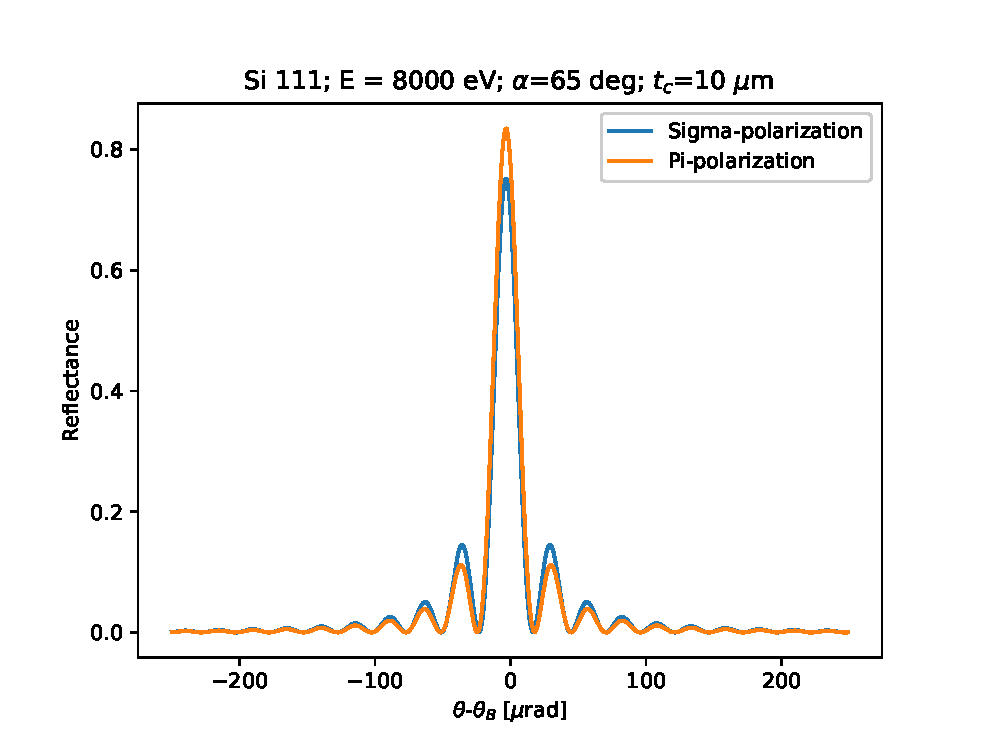
\includegraphics[width=0.49\textwidth]{figures/Laue_1.eps}
    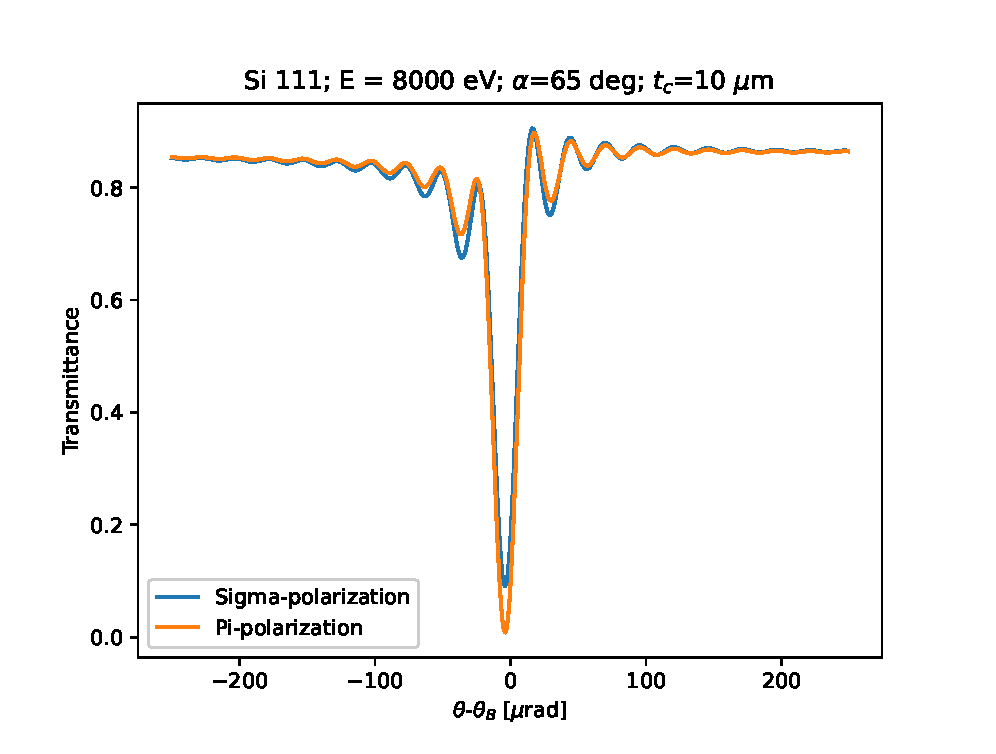
\includegraphics[width=0.49\textwidth]{figures/Laue_2.eps}
    \caption{Calculated reflectance and transmittance for a \SI{10}{\micro\meter} thick Laue Si 111 crystal  at 8 keV}.
\end{figure}

It is also interesting to consider the case of incidence along the direction of $\textbf{k}_h$ (diffraction vector $-\textbf{h}$), for which ($D_0(0), D_h(0)=(0,1)$. It is directly seen from equation~(\ref{eq:Mtransfer}) that the transmission and reflection amplitudes are $\bar{t}_L=m_{22}$ and $\bar{r}_L=m_{12}$ (note that the power factor will be $|b|$ in this case). These results can be written as

\begin{equation}\label{eq:MtransferLaue}
    \begin{pmatrix}
    t_L & \bar{r}_L\\
    r_L & \bar{t_L}
    \end{pmatrix}
    =
    \begin{pmatrix}
    m_{11} & m_{12}\\
    m_{21} & m_{22}
    \end{pmatrix}
    = M.
\end{equation}
This means that for the Laue case the matrix $M$ can be considered as the ``transfer-matrix" of the crystal slab, as well as the ``scattering-matrix" ($S$-matrix) which relates the vacuum waves leaving the crystal to the vacuum waves entering it. The term $S$-matrix is usual in the general scattering theory.  

Note that $u_{0,h,-h}$, $\omega$ and $a$ in equations~(\ref{eq:lauerandt}) are complex. The careful look at the real and imaginary parts leads to common expressions for absorption and Pendell\"osung. 

The exponential factor in equations~(\ref{eq:lauerandt}) gives a pure absorption term, which is (using $u_0 +\omega=[(b+1)u_0+b\alpha']/2$ from equation~({\ref{eq:omega}}), 
\inred{and setting $\alpha'=0 ???$}):  
\begin{subequations}
\begin{align}
   \inred{ \exp[\operatorname{Re}(-iT(u_0+\omega))] = }
    \exp[-T \frac{b+1}{2}\operatorname{Im}(u_0)] =  
    \exp[-T \frac{\pi}{\lambda}\frac{b+1}{2} \operatorname{Im} \chi_0].
\end{align}
\end{subequations}

The Pendell\"osung effect comes from the oscillations of $|\sin(aT)|^2$. Remembering the identity $|\sin(x+iy)|^2=\sin^2x + \sinh^2 y$, we get a Pendell\"osung distance (depending on $\theta$) along $s_0$ equal to  
$\pi / |\operatorname{Re} a|=\lambda / \operatorname{Re}\sqrt{b\chi_h\chi_{-h} + w^2}$.
At $\theta=\theta_c$, $b \chi_h \chi_{-h}+w^2=b \chi_h \chi_{-h} - [(1/2)(b-1)\operatorname{Im}\chi_0]^2$. In symmetric Laue case ($b$=1) we obtain the well-known formula of the Pendell\"osung distance along the direction normal to the crystal surface
\begin{equation}\label{eq:Pendellosung}
    \Lambda =\frac{\lambda}{\operatorname{Re}\sqrt{\chi_h\chi_{-h}}} \cos\theta_B.
\end{equation}

%%%%%%%%%%%%%%%%%%%%%%%%%%%%%%%%%%%%%%%%%%%%%%%%%%%%
%
%%%%%%%%%%%%%%%%%%%%%%%%%%%%%%%%%%%%%%%%%%%%%%%%%%%%
\subsection{\inred{Reflectance, transmittance and S-matrix} in the Bragg case (reflection geometry)}
\label{sec:TTsolutionsBragg}

In this case $b<0$. $T$ is, again, the path length in the crystal of the incident beam along $\textbf{k}_0$.
Setting $D_0(0)=1$ and $D_h(T)=0$ (which means no incident beam on the back surface of the crystal slab) in equation~(\ref{eq:Mtransfer}), we get for the reflection amplitude  $D_h(0)=r_B$ and the transmission amplitude $D_0(T)=t_B$, the relation $t_B=m_{11}+r_B m_{12}$ and $m_{21} + m_{22} r_B=0$. Therefore
\begin{equation}
    r_B = -\frac{m_{21}}{m_{22}} \text{ and } t_B = m_{11}-\frac{m_{12} m_{21}}{m_{22}}.
\end{equation}
Similarly, in the case of incidence on the crystal back side along the direction $\textbf{k}_h$ (diffraction vector $-\textbf{h}$), we set in equation~(\ref{eq:Mtransfer}) $D_h(T)=1$, $D_0(T)=\bar{r}_B$, $D_0(0)=0$ and $D_h(0)=\bar{t}_B$. We thus obtain $\bar{r}_B=m_{12} \bar{t}_B$ and $m_{22} \bar{t}_B=1$. Therefore 
\begin{equation}
    \bar{t}_B = \frac{1}{m_{22}} \text{ and } \bar{r}_B = \frac{m_{12}}{m_{22}}.
\end{equation}

Consequently, $S$-matrix for the Bragg case is represented as 
\begin{equation}\label{eq:scatteringMatrixDefinition}
    \begin{pmatrix}
    D_0(T)\\
    D_h(0)
    \end{pmatrix}
    =
    S
        \begin{pmatrix}
    D_0(0) \\
    D_h(T)
    \end{pmatrix},
\end{equation}
with
\begin{equation}\label{eq:scatteringMatrix}
    S = 
    \begin{pmatrix}
    s_{11} & s_{12}\\
    s_{21} & s_{22}
    \end{pmatrix}
    =
    \begin{pmatrix}
    m_{11}-\frac{m_{12} m_{21}}{m_{22}} & 
    \frac{m_{12}}{m_{22}}\\
    -\frac{m_{21}}{m_{22}} & 
    \frac{1}{m_{22}}
    \end{pmatrix}
    =
    \begin{pmatrix}
    t_B& 
    \bar{r}_B\\
    r_B& 
    \bar{t}_B
    \end{pmatrix}.
\end{equation}
Particularly, using equations~(\ref{eq:MtransferElements}),
\begin{subequations}
\label{eq:braggrandt}
\begin{empheq}[box=\fbox]{align}
r_B = s_{21}=
\frac{-i b u_h \sin(a T)}{a \cos(a T) + i \omega \sin(a T)}\\
t_B = s_{11}=
\frac{a~\exp(i T(u_0+ \omega))}{a \cos(a T) + i \omega \sin(a T)} ,
\end{empheq}
\end{subequations}

The diffraction profiles are $\mathcal{R}=|r|^2 P$ (diffracted intensity or reflectance) and $\mathcal{T}=|t|^2$ (forward diffracted intensity or transmittance).
An example is in Fig.~\ref{fig:braggProfiles}. 

\begin{figure}\label{fig:braggProfiles}
    \centering
    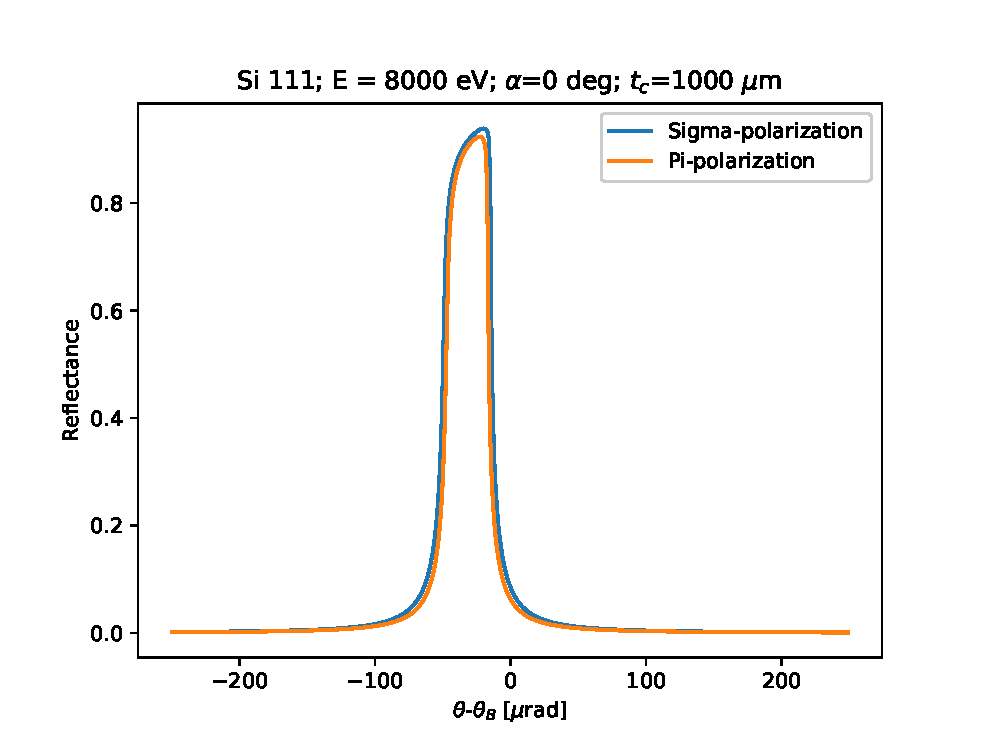
\includegraphics[width=0.49\textwidth]{figures/Bragg_1.eps}
    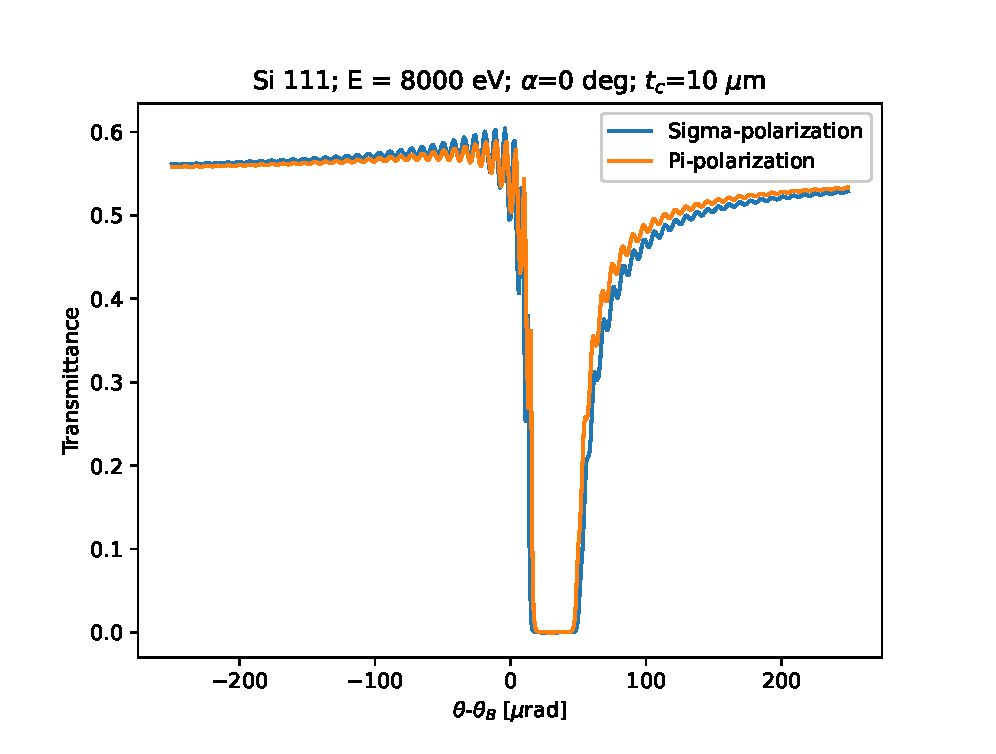
\includegraphics[width=0.49\textwidth]{figures/Bragg_2.eps}
    \caption{Example of reflected and transmitted intensities for a Bragg Si 111 crystal of $t_c=$\SI{10}{\micro\meter} at 8 keV. }
\end{figure}

It may be interesting to calculate the field inside the crystal, i.e. $D_0(s)$ and $D_h(s)$. Using equations (\ref{eq:BSolutions}), with $D_0(0)=1$ and $D_h(0)=r_B$ from equation (\ref{eq:braggrandt}a) we obtain
\begin{subequations}\label{eq:bragginside}
\begin{align}
D_h(s)&=\frac{i b u_h \sin(as - aT)}{a \cos(aT) + i \omega \sin(aT)} e^{is(u_0+\omega)} 
= r_B \frac{\sin(as - aT)}{\sin(aT)} e^{is(u_0+\omega)}\\
D_0(s)&= \frac{a \cos(as-aT) - i \omega \sin(as-aT)}{a \cos(aT) + i \omega \sin(aT)} e^{is(u_0+\omega)}.
\end{align}
\end{subequations}

An example of simulation of the field inside the crystal using equations~(\ref{eq:bragginside}) is in Fig.~\ref{fig:braggMap}. For the Laue case, also shown in this figure, we observe that the field at coordinate $s$ is simply calculated by the equations~(\ref{eq:lauerandt}) replacing $T$ by $s$.

\begin{figure}\label{fig:braggMap}
    \centering
    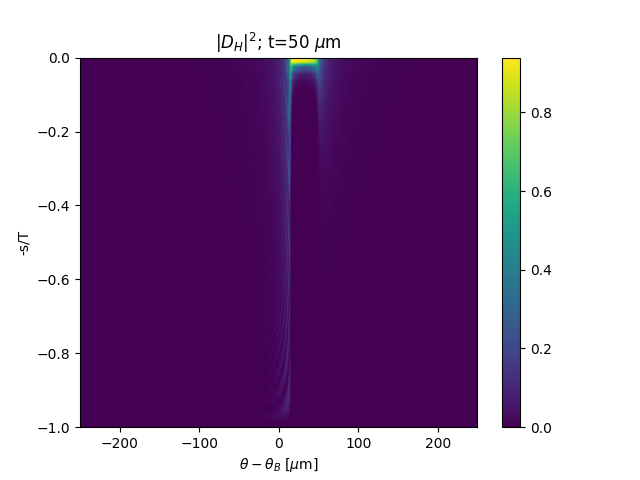
\includegraphics[width=0.49\textwidth]{figures/Bragg_DH.png}
    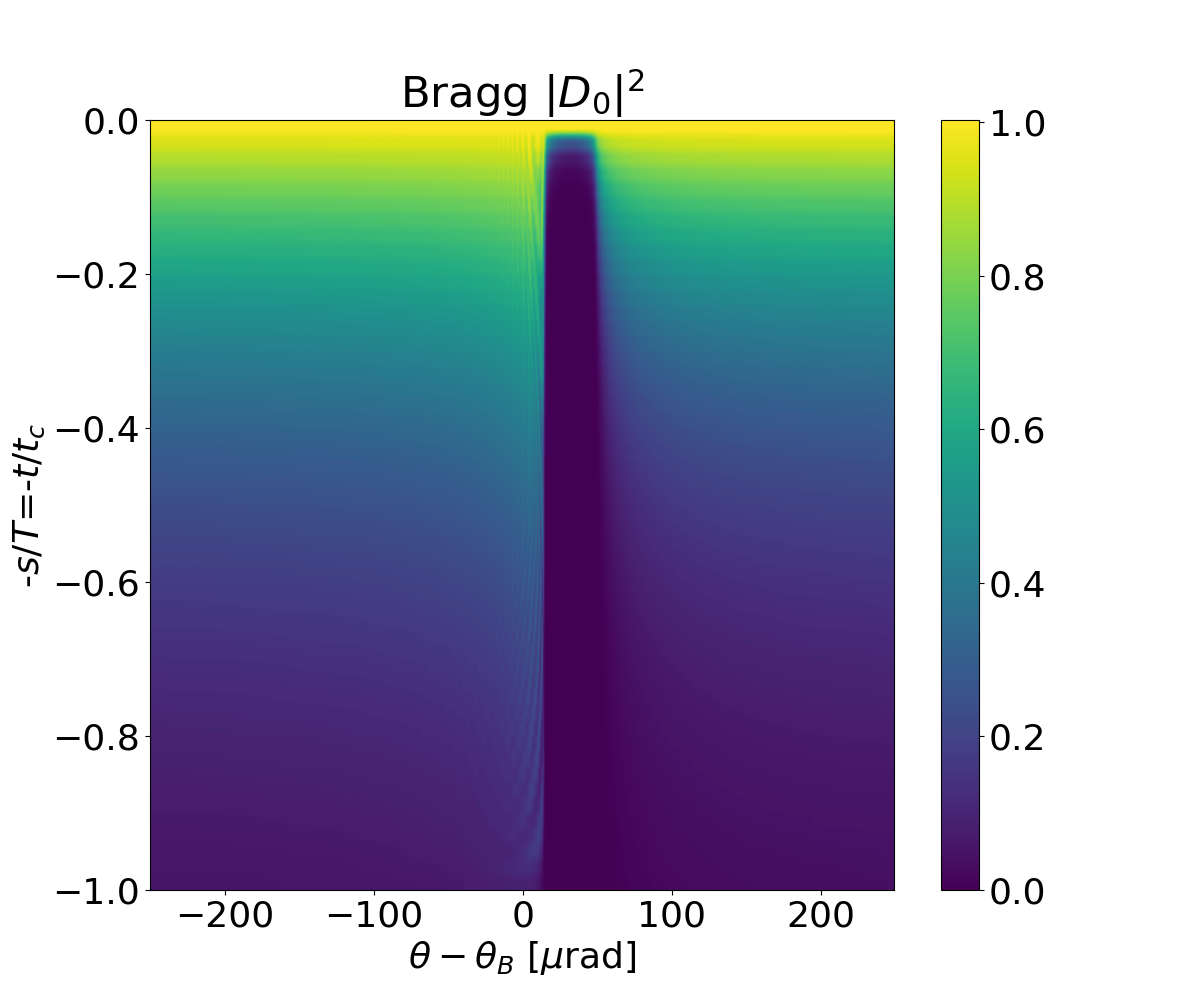
\includegraphics[width=0.49\textwidth]{figures/Bragg_D0.png}
    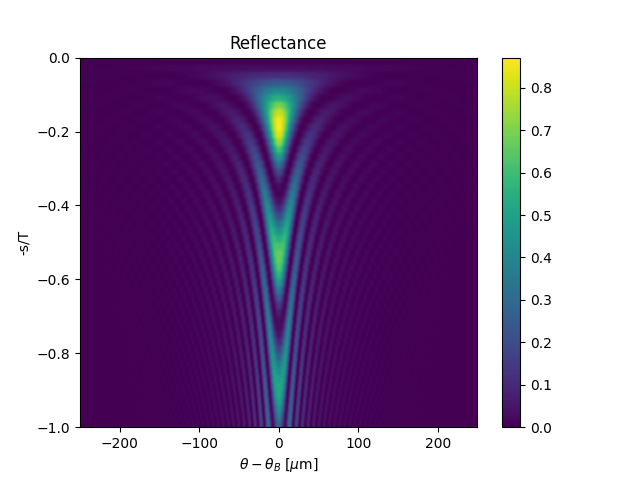
\includegraphics[width=0.49\textwidth]{figures/Laue_DH.png}
    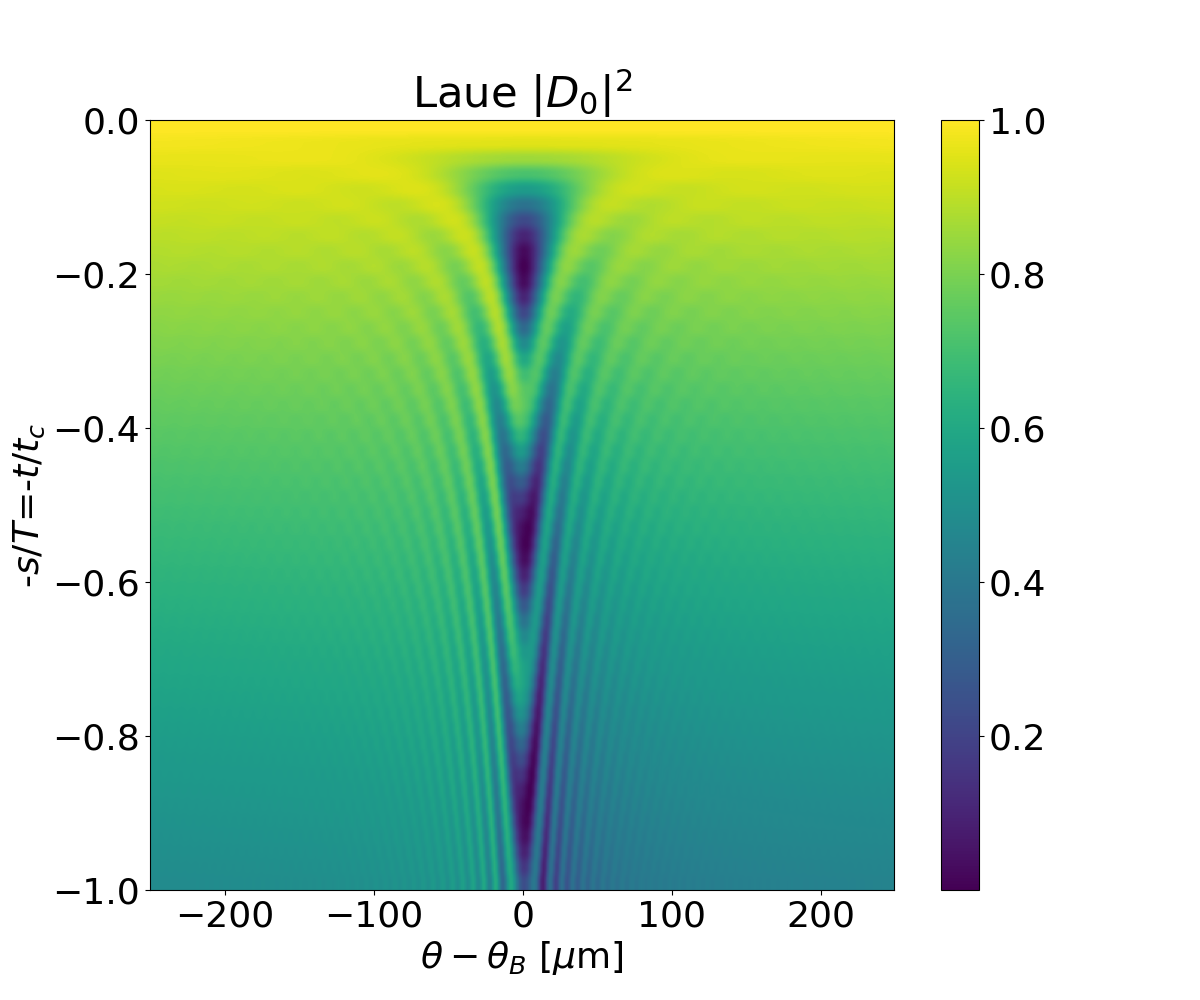
\includegraphics[width=0.49\textwidth]{figures/Laue_D0.png}
    \caption{Examples of electric field intensity inside the crystal as a function of the 
    deviation angle $\theta-\theta_B$ and thickness ratio $-s/T$ for a symmetric Si 111 at 8 keV with thickness $t=$\SI{50}{\micro\meter} in Bragg or Laue geometry. 
    a) Bragg $|D_h|^2$, b) Bragg $|D_0|^2$,
    c) Laue $|D_h|^2$, d) Laue $|D_0|^2$.
    \todo{Change the titles for consistency}
    }
\end{figure}




% \todo{Discuss also the case of a thick crystal with a capping crystal layer. The final transfer matrix is then $M$ for the capping layer multiplied by the $M$ of the thick substrate...}

% \section{Scattering and transfer matrices}
% \label{sec:matrices}

% Equations (\ref{eq:BSolutions}) represent a system of two equations containing two coefficients $c_1$ and $c_2$ and two fields ($B_0$ and $B_h$) that are latter expressed at the top ($s=0$) and bottom ($s=T$) surfaces. From these four fields, we can calculate two as a function of the other two. In the usual case, we calculate the diffracted and transmitted fields at the corresponding exit surface (which depends on the geometry, Bragg or Laue) given the other two that are set as boundary conditions. This gives the ``scattering matrix". In other cases, when one considers a complex crystal made by several piled individual crystal layer, we would be interested in calculating the diffracted and transmitted beam at the bottom as a function of the beams from the top.   

% \subsection{Scattering matrix in Bragg case}
% For the Bragg case, we calculate $D_0(T)$ (transmitted) and $D_h(0)$ (diffracted) as a function of generic $D_0(0)$ and $D_h(T)$, so we can write in matrix form
% \begin{equation}
%     \begin{pmatrix}
%     D_h(0)\\
%     D_0(T)
%     \end{pmatrix}
%     =
%     S
%         \begin{pmatrix}
%     D_0(0) \\
%     D_h(T)
%     \end{pmatrix}
%     =
%     \begin{pmatrix}
%     s_{11} & s_{12}\\
%     s_{21} & s_{22}
%     \end{pmatrix}
%     \begin{pmatrix}
%     D_0(0) \\
%     D_h(T)
%     \end{pmatrix},
% \end{equation}
% where the terms of the scattering matrix $S$ are 
% \begin{subequations}\label{eq:scatteringMatrix }
% \begin{align}
% s_{11} &= \frac{-i b u_h \sin(a T)}{a \cos(a T) + i \omega \sin(a T)};\\
% s_{12} &= \frac{a~\exp(-i T (u_0+ \omega))}{a \cos(a T) + i \omega \sin(a T)};\\
% s_{21} &= \frac{a~\exp(i T (u_0+ \omega))}{a \cos(a T) + i \omega \sin(a T)};\\
% s_{22} &= \frac{-i u_{-h} \sin(a T)}{a \cos(a T) + i \omega \sin(a T)}.
% \end{align}
% \end{subequations}


% For the case studied in section~\ref{sec:TTsolutionsBragg} we set $(D_0(0),D_h(T))=(1,0)$ from there we get $s_{11}=r; s_{21}=t$, with $r$ and $t$ from equations (\ref{eq:braggrandt}). 

% % Similarly, when the incident beam enters the crystal by the bottom surface, as studied in appendix~\ref{sec:braggfromtheback}, we set $(D_0(0),D_h(T))=(0,1)$ and  we get $s_{12}=\bar{r}; s_{22}=\bar{t}$, with $r$ and $t$ from equations (\ref{eq:braggrbarandtbar}) \todo{suppress the appendix?}.


 % \todo{Move this section to ``Bragg section", and obtain these results from the $M$ for the thick crystal}




\inred{
In case of thick Bragg crystal, the reflection amplitude is given by $r_B=-m_{21}/m_{22}$ which from equation~(\ref{eq:Mthickapprox}) gives  
\begin{equation}\label{eq:thickbraggr}
    r_B^{\text{thick}} = \frac{b u_h}{a-\omega} = \frac{a+\omega}{u_{-h}},
\end{equation}
where $a$ can be obtained from $a^2$ as: 
\begin{equation}
a = \frac{1}{\sqrt{2}} \left[ \frac{\operatorname{Im}(a^2)}{\sqrt{|a^2|-\operatorname{Re}(a^2)}} + i \sqrt{|a^2|-\operatorname{Re}(a^2)} \right].
\end{equation}

Equation~(\ref{eq:thickbraggr}) is a useful result, as most crystal monochromators used in synchrotron radiation are thick crystals in Bragg (reflection) mode. 

% For all other geometries (Bragg transmission, and both Laue cases) the approximation $T\rightarrow \infty$ makes the exponential term tends to zero, therefore there is no intensity at the back crystal surface. If we apply the approximations mentioned, but leave the exponential term (with a reasonable small $T$, thus small absorption), we obtain diffraction intensity distributions that do not present Pendell\"osung. The simplified form of equation~ (\ref{eq:braggrandt}b) is   
% \begin{equation}\label{eq:thickbraggt}
%     t_B = \frac{2a}{a-\omega} e^{i T (u_0+\omega+a)},
% \end{equation}
% and for the Laue case [equations (\ref{eq:lauerandt}b)] we get
% \begin{subequations}
% \label{eq:thicklaue}
% \begin{align}
% r_L = & - \frac{b u_h}{2 a} e^{iT (u_0+\omega-a)}  \\
% t_L = & \frac{1}{2} (1 + \frac{\omega}{a})e^{i T (u_0+\omega-a)}.
% \end{align}
% \end{subequations}

}


%%%%%%%%%%%%%%%%%%%%%%%%%%%%%%%%%%%%%%%%%%%%%%%%%%%%
%
%%%%%%%%%%%%%%%%%%%%%%%%%%%%%%%%%%%%%%%%%%%%%%%%%%%%
\subsection{\inred{Calculation of raflection and transmission amplitudes using the transfer matrix}}

The matrix method permits to obtain the complex reflection and transmission amplitudes of a crystal made by layers of different crystals (or the same crystal with different orientations). For that,
i) construct the transfer matrix of the total crystal by multiplication\footnote{\inred{The multiplication be from bottom to top, i.e. $M=M_n M_{n-1}...M_2 M_1$}}
of the transfer matrices of the different layers [each one calculated using equations~(\ref{eq:MtransferElements})];
ii) if geometry is Laue, obtain reflectance and transmittance using the coefficients $m_{21}$ and $m_{11}$ of this matrix [equation~(\ref{eq:lauerandt})], respectively; otherwise (Bragg geometry), compute the scattering matrix using equation~(\ref{eq:scatteringMatrix}) and reflectance and transmittance are given in the matrix terms $s_{21}$ and $s_{11}$ [equation~(\ref{eq:braggrandt})], respectively.

\inred{A first example shows how simple is to apply this recipe of multiplication of transfer matrices to get the reflectance of a simple two-layer crystal. Consider}
a bilayer of two identical crystal layers of thickness $T$ and transfer matrix $M$ for each one. Using matrix analysis, the transfer matrix of the bilayer is $[M(T)]^2=M(2T)$ from which is easy to compute the reflectivity in Bragg geometry [equation~(\ref{eq:braggrandt})]. Otherwise, if this result would be obtained via the reflectivities ($r$ and $\bar{r}$) and transmittivities ($t$ and $\bar{t}$) of the single layer (S-matrix), the reflectivity of the bilayer results from an infinite series as shown in  Fig.~\ref{fig:doublelayer}.
 
\begin{figure}\label{fig:doublelayer}
    \centering
    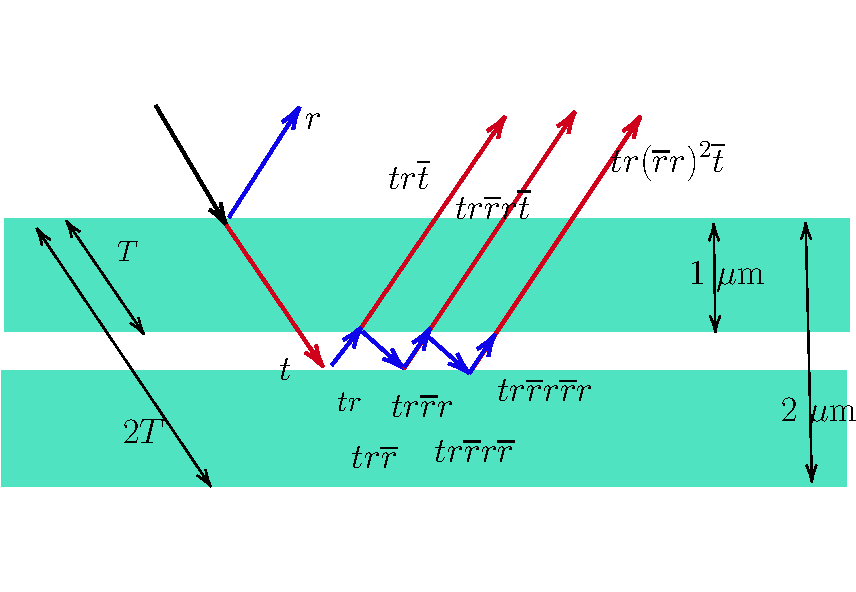
\includegraphics[width=0.49\textwidth]{figures/figlayered2.pdf}
    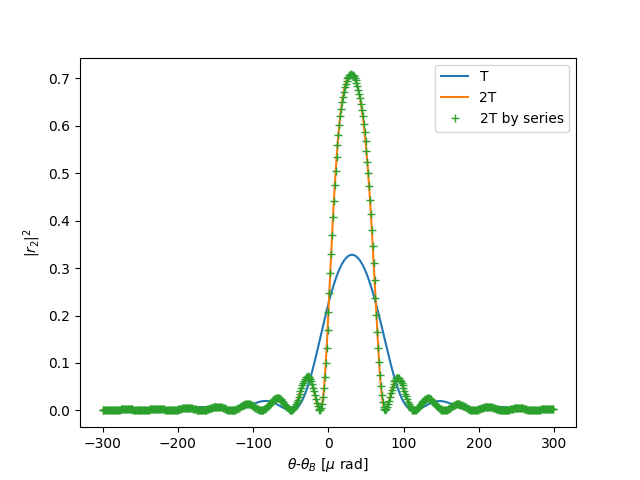
\includegraphics[width=0.49\textwidth]{figures/doublelayer2.png}
    \caption{Example of calculation of the reflection amplitude $r_2$ of a Si 111 crystal of \SI{2}{\micro\meter} thickness from the amplitudes of the half-layer (\SI{1}{\micro\meter}). The reflectivity of the bilayer $r_2$ can be obtained as an infinite sum $r_2 = r + r t \bar{t} + r t \bar{t} (r \bar{r}) + r t \bar{t} (r \bar{r})^2 + ...= r[1 + t \bar{t}\sum_{n=0}^{\infty}(r\bar{r})^n]=r(1 + (t \bar{t} / (1-r \bar{r})))$. Calculations done with {\tt crystalpy} for a photon energy of 8 keV..}
\end{figure}


A second example is the Bragg reflection of a crystal layer on a thick substrate. The transfer matrix of the set $M'$ is calculated as
\begin{equation}
    M' = M^{\text{thick}} \times M,
\end{equation}
with $M^{\text{thick}}$ the transfer matrix of the substrate and $M$ the transfer matrix of the thin layer. We are interested in the Bragg reflectance or 
\begin{equation}
r_B=-\frac{m'_{21}}{m'_{22}}=
-\frac{m_{21}^{\text{thick}} m_{11} + m_{22}^{\text{thick}} m_{21}}
{m_{21}^{\text{thick}} m_{12} + m_{22}^{\text{thick}} m_{22}}.
\end{equation}
This can be expressed as a function of the substrate reflectance $r_S=-m_{21}^{\text{thick}}/m_{22}^{\text{thick}}$ giving: 
\begin{equation}
r_B=\frac{r_S m_{11} - m_{12}}
{m_{22}  - r_S m_{11}}.
\end{equation}

 The method of transfer matrix multiplication can also be used for analyzing distorted and bent crystals and will be explored in a future work.
%%%%%%%%%%%%%%%%%%%%%%%%%%%%%%%%%%%%%%%%%%%%%%%%%%%%
%
%%%%%%%%%%%%%%%%%%%%%%%%%%%%%%%%%%%%%%%%%%%%%%%%%%%%

\subsection{The direction of the incident and diffracted waves}\label{sec:directions}
\inblue{
As mentioned before, the selection of the directions used to solve the TT equations contains some dose of arbitrarily. In our choice, $\textbf{k}_0$ vector corresponds exactly with the direction and wavelength of the incident ray or wave, which is not necessarily verifying the Bragg law.
The vector $\textbf{k}_h$ (see section~\ref{sec:TT}) is defined as as $\textbf k_h=\textbf k_0 + \textbf h$. Therefore, it is not necessarily matching the wavevector of the outgoing ray or wave outside the crystal.
In many applications, like in ray tracing, it is essential to know the output wavevector $\textbf{k}_{\text{out}}$ that exits from the crystal. The length of $\textbf{k}_h$ is [equation~(\ref{eq:alpha})] $|\textbf{k}_h|=k\sqrt{1-\alpha}$.
To get $\textbf{k}_{\text{out}}$ we must get into account i) its length is the same as $\textbf{k}_0$, and ii) its value parallel to the crystal surface $\textbf{k}_{\text{out}, ||}$ must be equal to $\textbf{k}_{h,||}$ (continuity of the tangential component of the electric field at the crystal-vacuum interface).
These conditions permit to determine how the perpendicular component of $\textbf{k}_{\text{out}}$ differs from $\textbf{k}_h$
\begin{equation}
    \textbf{k}_{\text{out}, \bot} = \kappa \textbf{k}_{h,\bot},
\end{equation}
with 
\begin{equation}
    \kappa^2 = \frac{|\textbf{k}_0|^2-|\textbf{k}_{h,||}|^2}
    {|\textbf{k}_{h,\bot}|^2}
\end{equation}
}

\todo{simplify the discussion? Write $\textbf{k}_{\text{out}, \bot} = \text{something} \times \textbf{n}$? }

\todo{ something still not clear:

The formulation done is ``inside the crystal". Therefore $D_{0,h}(0)$ corresponds to the field ``inside" the crystal. So, $D_0(0)=1$ is the amplitude of the incident plane wave inside the crystal. 
And $\Psi_0(0)=D_0(0) e^{i \textbf{k}_0. \textbf{r}}$ with $\textbf{k}_0$ outside the crystal. This may be confusing but it is just definitions.  
Right? 

Having $\Psi(\textbf r) = D_0(\textbf r) e^{i \textbf k_0 . \textbf r} + D_h(\textbf r) e^{i \textbf k_h . \textbf r}$ this implies $\Psi(s) = D_0(s) e^{i \textbf k_0 . \textbf{s}} + D_h(s) e^{i \textbf k_h . \textbf s}$ with $\textbf{s}=(s_0,s_h)$. Can we write $\Psi(s)=\Psi_0(s)+\Psi_h(s)$?


For the output beam (in Bragg), we calculate $D_h(0)$ inside the crystal. The direction of the scattered wave is $\textbf{k}_{\textbf{out}}$ as defined before. 
Is it really necessary to use the conservation of the parallel component of the diffraction $\textbf{h}_{\textbf{out},||}= \textbf{k}_{0,||} + \textbf{h}_{||}$? Or, can it be deduced in another way, like using  $\nabla  \arg(\Psi_h(0))$? 

Other things: 
\begin{itemize}
    \item discuss the fact that $b$ is not constant.
    \item may be: make a comment for the grazing incidence case (\cite{Yashiro2001, Stepanov1998})
\end{itemize}
}

% \inred{
% \subsection{Application to multilayers}
% }\label{sec:multilayers}


% \todo{REMOVE THIS SECTION. LEFT FOR THE FUTURE?

% Can we directly apply the amplitudes in (\ref{eq:braggrandt}) to a multilayer? It is enough to replace $\chi_0$ by the averaged $\bar{\chi}=n^2-1$ and $\chi_h$ by $\chi_1$ and $\chi_{-h}$ by $\chi_{-1}$? Is this a bilayer? Shall we then use the scattering matrix? 
% Can we use $\alpha=2(\theta-\theta_B)\sin(2\theta_B)$ ?
% See also \cite{Osterhoff2012,Osterhoff2013}.

% Some possible ideas for the matrix methods
% \begin{itemize}
%     \item the multilayer case:
%     \begin{itemize}
%         \item relation between scattering and transfer matrices for multilayers. We can build a multilayered $M=\Pi M_i$ and then calculate its corresponding scattering matrix?
%         \item Connection with the Parratt recursion formula
%         \item transition layer (non-abrupt change, see \cite{Lobach})
%         \item Roughness layer
%     \end{itemize}and 
%     \item may be: discuss the roughness layer

% \end{itemize}
% }

% \inred{
% \subsection{OTHER SECTIONS?}
% }

% \todo{
% \begin{itemize}
%     \item Discuss the differences of the presented theory with Darwin (see \cite{Yashiro2000, Yashiro2001}), Ewald (??), Zachariasen (none, as seen in Appendix~\ref{appendix:zachariasen}), etc. 
% \end{itemize}
% }


%%%%%%%%%%%%%%%%%%%%%%%%%%%%%%%%%%%%%%%%%%%%%%%%%%%%
\section{The {\tt crystalpy} library}
\label{sec:crystalpy}


% For the moment, only flat perfect crystals are implemented in the {\tt PerfectCrystalDiffraction} class implementing the formulation and theory presented in section~\ref{sec:TTsolutions}. The {\tt PerfectCrystalDiffraction} class handles the actual computations. 





{\tt Crystalpy} is a Python library that performs calculations on diffraction
from perfect crystals using the formalism introduced in the previous chapters.
% It also simulates the changes in the polarization state of the x-ray beam brought about by the diffraction using Müller-Stokes formalism. 
% The first version of this library was developed by Edoardo Cappelli, Mark Glass and Manuel Sanchez del Rio. 
The motivation of {\tt crystalpy} 
was to create a modern, extensible, well-documented, and friendly library to overcome the difficulties of integrating ancient software tools based on the dynamical diffraction theory. It is specifically designed for two objectives: support for new versions of the crystal diffraction codes delivered in platforms like OASYS \cite{codeOASYS}, and provide a core for ray tracing simulations with crystals.  
The {\tt crystalpy} library is written in the python language and uses standard libraries (numpy and scipy). It makes use of vector calculus and stack operations to accelerate the calculations. Therefore, it is adapted for being used in ray tracing tools, such as the future SHADOW~\cite{codeSHADOW} versions. 
% It basically contains three packages: {\tt util}, {\tt diffraction} and {\tt polarization}.

To simulate a diffraction experiment using a perfect crystal, {\tt crystalpy}  offers functions that implement the theory described previously. Two input objects must be prepared: i) the incident wave(s) or  photon ray(s), and ii) the information on the crystal (diffraction setup). The objects representing these two entities are described here. 

The {\tt Photon} class is a minimum class for a photon, containing the energy (in eV) and a unit direction vector, implemented in 
the {\tt Vector} class. It deals with the storage and operations (addition, scalar product, cross product, normalization, rotation around an axis, etc.) of a 3D vector. A superclass of {\tt Photon} is {\tt ComplexAmplitudePhoton}, that contains the scalar complex amplitude for $\sigma$ and $\pi$ polarizations). 
These classes ({\tt Vector}, {\tt Photon} and {\tt ComplexAmplitudePhoton}) can hold stacks (the internal storage is done with arrays to speed-up vector operations). The {\tt ComplexAmplitidePhoton} classes 
has a corresponding {\tt ComplexAmplitudePhotonBunch} superclass, decorated with methods to deal with multiple waves or beams (bunches or sets of photons). 

The information on the crystal itself (e.g., particular crystal material and crystal structure), its preparation (crystal cut), and related physical parameters (like the structure factor) are managed by the {\tt DiffractionSetup} classes. {\tt Crystalpy} allows multiple options to retrieve the crystal structure and the scattering functions needed to calculate the structure factors. 
The {\tt DiffractionSetupAbstract} class defines the methods to access the basic information of the crystal (defined as a string, e.g. ``Si") such as {\tt angleBragg}, {\tt dSpacing}, and {\tt unitCellVolume}, and to compute the structure factors: {\tt F0}, {\tt FH}, {\tt FH\_bar}. These parameters can be obtained from several libraries external to {\tt crystalpy}. We implemented three options: i) {\tt DiffractionSetupXraylib} using the {\tt xraylib} library \cite{xraylib}, ii) {\tt DiffractionSetupDabax} that uses the DABAX library \cite{dabax}, and iii) using an ad-hoc generated data file. This modular structure permits disconnecting the calculation part from the access to optical and physical constants. Indeed, when using ad-hoc data files we do not have to import {\tt xraylib} or {\tt dabax} packages. We implemented this for the crystal material files of the SHADOW~\cite{codeSHADOW} code in the traditional version ({\tt DiffractionSetupShadowPreprocessorV1}), and in a more recent version \cite{Yu2022} supporting high d-spacing crystals ({\tt DiffractionSetupShadowPreprocessorV2}).
The {\tt DiffractionSetup} classes handle the information about the crystal setup and collects all the parameters needed to fully define the physical system we are modelling:
{\tt geometry\_type} (among {\tt BraggDiffraction, BraggTransmission, LaueDiffraction} and {\tt LaueTransmission}),
{\tt crystal\_name} (a string, e.g. Si, Ge),
{\tt thickness} (crystal thickness in SI units [m]),
{\tt miller\_h(,k,l)} (the Miller indices),
and {\tt asymmetry\_angle} (angle in degrees between the crystal surface and the planes $hkl$ as defined in \cite{codeCRYSTAL}).
% shown in figure~\ref{fig:edo_sketch}).

To perform the main calculations (reflectivities, transfer matrices, diffracted photons, etc.) several methods in the {\tt Diffraction} class are used, getting the crystal setup and the photon bunch as inputs. For the moment, only flat perfect crystals are coded (in the {\tt PerfectCrystalDiffraction} class) which directly implements the formulation and theory in section~\ref{sec:TTsolutions}. For completeness, {\tt crystalpy} also includes the equations of the Zachariasen formalist~\cite{ZachariasenBook} and can be used instead of the ones described in this paper.
Typical angle or photon scans as shown in Fig.~\ref{fig:braggProfiles} are calculated defining a $\tt ComplexAmplitudePhoton$ entity for each point, group then in a {\tt ComplexAmplitudePhotonBunch} for then calculate the diffraction by the crystal using {\tt calculateDiffractedComplexAmplitudes}. \todo{listing?} 

A user-friendly application has been written in the OASYS environment to compute diffraction profiles using {\tt crystalpy} (Fig.~\ref{fig:xcrystal}). The applications automatically generates a script that can be used for further batch calculations. 

\begin{figure}
    \centering
    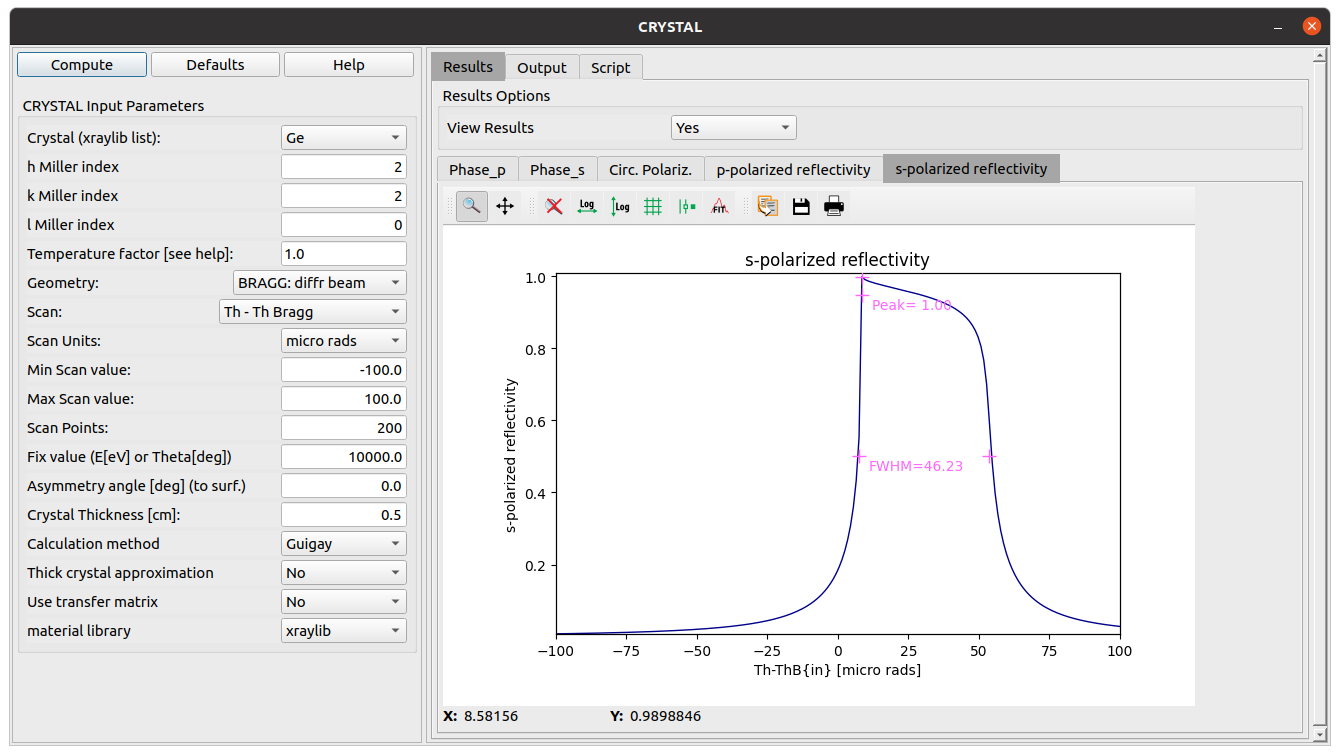
\includegraphics[width=0.8\textwidth]{figures/xcrystal.png}
    \caption{Interactive application for computing the perfect crystal diffraction profiles using {\tt crystalpy} and available in OASYS.  }
    \label{fig:xcrystal}
\end{figure}


In the ray tracing SHADOW4, all calculations related to crystal optics are delegated to  {\tt crystalpy}. Ray tracing permits simulations of beamline optics including a realistic description of the source. It also allows the simulation of curved crystals, under the assumption that the local reflectivity of the curved crystal is the same as for the flat crystal. This assumption is not always granted and has to be verified before ray tracing curved crystals. \todo{Example?}


\todo{
\begin{itemize}
    \item a high numerical precision is required for calculating $\sin(aT)$, $\cos(aT)$ and $\exp(iT(u_0+\omega))$ for large values of T. This is  a typical problem when calculating Bragg reflection case using a large $t_c$. Can we make a recipe to switch to the "thick" crystal model for $t_c>t_{\text{eff}}$. How to calculate $t_{\text{eff}}$? 
\end{itemize}
}

% \begin{figure}
%     \centering
%     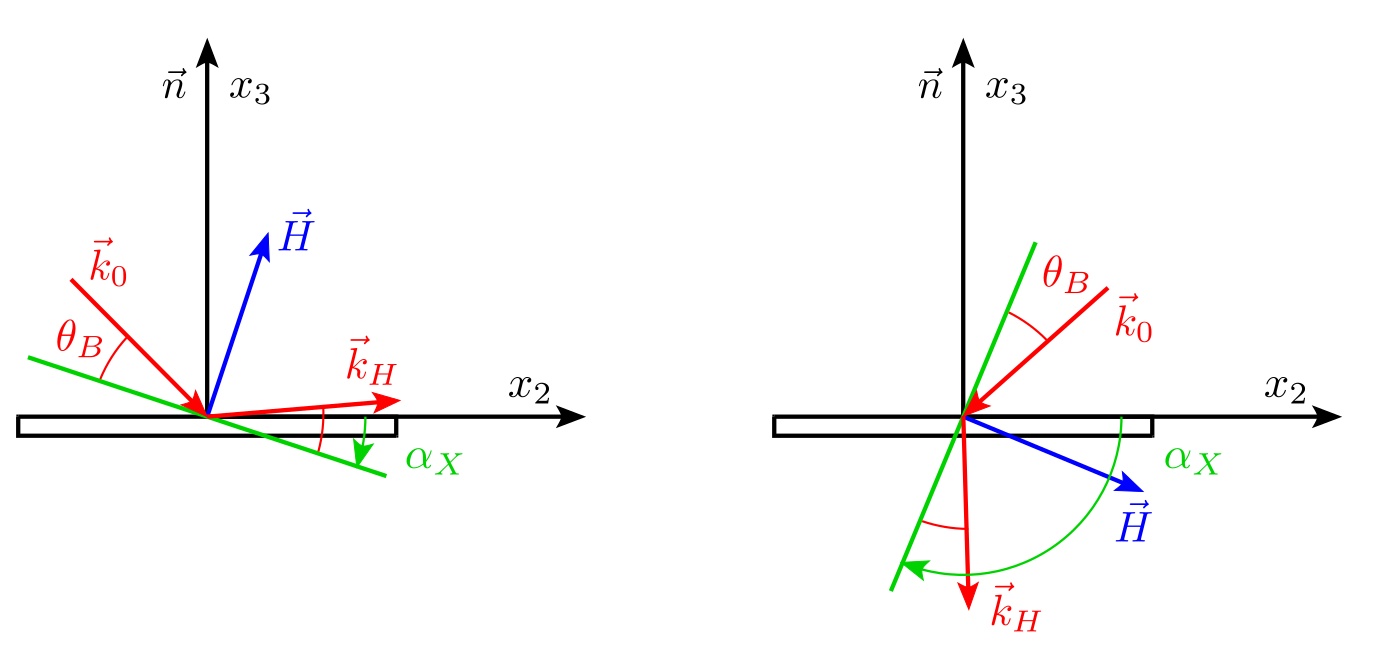
\includegraphics[width=0.8\textwidth]{figures/edo_sketch.png}
%     \caption{Schematic drawings of Bragg (left) and Laue (right) diffraction setups: \textbf{H} is the reciprocal vector associated with the $hkl$ family of lattice planes, also called the Bragg normal, $\theta_B$ is the Bragg angle and $\alpha_X$ is the asymmetry angle as discussed in \cite{codeCRYSTAL}.
%     \todo{change vector format (from arrows to bold)} }
%     \label{fig:edo_sketch}
% \end{figure}

% As examples of the use of {\tt crystalpy}, we should mention that the figures shown in this work are calculated with {\tt crystalpy}: diffraction profiles (see Figs.~\ref{fig:braggProfiles}, \ref{fig:laueProfiles}); and field maps inside the crystal using equation~(\ref{eq:bragginside}). 


% \todo{ 
% \begin{itemize}
%     \item Describe the Polarization/Muller functionality
%     \item loot at the inwards/outwards normal (in the code it is still outwards...)
%     \item discuss the numerical precision 
% \end{itemize}
% }

% \todo{ 
% Other examples that may be discussed: 
% \begin{itemize}
%     \item discuss that we calculate the matrices for both s and p-polarization. Calculate phase (polarization) changes [implement a phase-retarder example]
%     \item skew scans (2D scans) [Needs to calculate the output direction]
% \end{itemize}
% }

\section{Conclusions and future perspectives}
\label{sec:summary}

We have presented a theoretical and numerical description of the dynamical diffraction in perfect crystals. In the first part of this paper, we presented a new perspective of the well-known dynamical theory of diffraction applied to undeformed perfect crystals. We deduced the equations of diffraction amplitudes (as well as intensity reflectance and transmittance) starting from basic principles via the solution of the Takagi-Taupin equations. We calculated the transfer matrix, useful to compute the diffraction of stacked crystal layers, and also the scattering matrix, of interest for the Bragg case. For completeness, our results are compared to those presented in the well-known textbook by \cite{ZachariasenBook} (see appendix~\ref{appendix:zachariasen}).
In the second part we presented {\tt crystalpy}, a software library completely written in python that implements the theory previously discussed. This open source tool can be used to predict the diffraction properties of any crystal structure, like Si, Ge or diamond typically used in synchrotron beamlines, but also for any other crystal provided its crystalline structure. This library is intended to replace multiple scattered pieces of software in packages like OASYS \cite{codeOASYS} and is designed to be the kernel of the crystal calculations in a new version of the SHADOW \cite{codeSHADOW} ray tracing code. The crystalpy library and its documentation are available from \url{https://github.com/oasys-kit/crystalpy}. 


% \ack{Acknowledgements}
% A large part of this work comes from ...


\bibliography{iucr} % reads iucr.bib with items
\bibliographystyle{iucr}
%\referencelist{library}

\appendix

\section{Derivation of the TT equations for a rotating perfect crystal}
\label{appendix:rotating}

In the ``rotating crystal mode", the crystal is rotated around an axis perpendicular to the ``diffraction plane" which contains the diffraction vector $\textbf{h}$ and the wave-vector $\textbf{k}_0$ of the fixed incident plane-wave in vacuum. The crystal rotation from the exact geometrical Bragg position may be viewed as a special kind of crystal deformation. We propose to use the Takagi-Taupin approach to derive some basic results of the usual dynamic theory for perfect crystal diffraction. 

The x-ray wavefield inside the crystal is set as
\begin{subequations}
\label{eq:wavefieldappendix}
\begin{align}
        \Psi(\textbf r) = 
        e^{i \textbf k_0 . \textbf r} \left[
        A_0(\textbf r) + e^{i \textbf k_{B} . \textbf r} A_h(\textbf r)
        \right] = 
        \nonumber\\
        A_0(\textbf r) e^{i \textbf k_0 . \textbf r} + A_{h}(\textbf r) e^{i \textbf k_{hB} . \textbf r},
\end{align}
\end{subequations}
$\textbf{h}_B$ representing the diffraction vector in exact Bragg position. The vector $\textbf k_{hB}$  is therefore such that $|\textbf k_{0}|=|\textbf k_{hB}|=k=2 \pi / \lambda$. The Fourier coefficients $\chi_h$ of the perfect crystal susceptibility are \cyan{to be} replaced by the function $\chi_h \exp[i\textbf{k}_b.\textbf{u}(\textbf{r})]$, in which $\textbf{u}(\textbf{r})$ is the displacement field of the rotated crystal. The phase term $\exp[i\textbf{h}_B.\textbf{u}(\textbf{r})]$ will be written as $\exp(i\phi(\textbf{r})$. In such conditions, the following form of the TT equations
\begin{subequations}
\label{eq:TTvectorappendix}
\begin{align}
2 i \textbf{k}_0 . \nabla A_0 + \chi_0 k^2 A_0 + \chi_{-h} k^2 \exp(i\phi) A_h =& 0; \\
2 i \textbf{k}_{hB} . \nabla A_h + \chi_0 k^2 A_h + \chi_{h} k^2 \exp(-i\phi) A_0 =& 0,
\end{align}
\end{subequations}
is obtained by inserting this expression in the \cyan{Helmholz equation~(\ref{eq:helmholz})}, with the following approximations: the 2$^{\text{nd}}$-order derivatives of $A_{0,h}$ supposed to be slowly varying amplitudes are neglected and only the terms containing $\exp(i\textbf{k}_0.\textbf{r})$ in the product $\chi\Psi$ are considered. Introducing oblique coordinates $(s_0,s_h)$ in the diffraction plane, along the directions $\textbf{k}_0$ and $\textbf{k}_{hB}$, so that $\textbf{k}_0.\nabla A_0=k\frac{\partial A_0}{\partial s_0}$ and  $\textbf{k}_{hB}.\nabla A_h=k\frac{\partial A_h}{\partial s_h}$, the TT equations are
\begin{subequations}
\begin{align}
\frac{\partial A_0}{\partial s_0} =& \frac{ik}{2} \left[ \chi_0 A_0+ \chi_{-h} \exp(i\phi) A_h\right]; \\
\frac{\partial A_h}{\partial s_h} =& \frac{ik}{2} \left[ \chi_0 A_h+ \chi_{\cyan{h}} \exp(-\phi) A_0\right].
\end{align}
\end{subequations}

Performing the transformation $A_0=D_0$ and $\exp(i\phi) A_h=D_h$, we obtain
\begin{subequations}
\begin{align}
\frac{\partial D_0}{\partial s_0} =& \frac{ik}{2} \left[ \chi_0 D_0+ \chi_{-h} D_h\right]; \\
\frac{\partial D_h}{\partial s_h} =& \frac{ik}{2} \left[ (\chi_0 + \frac{2}{k}\frac{\partial\phi}{\partial s_h} ) D_h+ \chi_{\cyan{h}} D_0\right].
\end{align}
\end{subequations}
This is identical to equation~(\ref{eq:TT}) considering that $\alpha=\frac{2}{k}\frac{\partial\phi}{\partial s_h}$, \cyan{which demonstration follows.}

\subsection{Demonstration of $\alpha=\frac{2}{k}\frac{\partial\phi}{\partial s_h}$ }

Let $\textbf{i}_{0,h}$ be unit vectors along the directions of $\textbf{k}_0$ an $\textbf{k}_{hB}$; the crystal rotation $\Delta\theta=\theta-\theta_B$ transforms $\textbf{i}_{0,h}$ into $\textbf{j}_{0,h}$. A position vector $s_0\textbf{i}_0+s_h\textbf{i}_h$ is transformed into $s_0\textbf{j}_0+s_h\textbf{j}_h$. The displacement field is $\textbf{u}(s_0,s_h)=s_0(\textbf{j}_0-\textbf{i}_0)+ s_h(\textbf{j}_h-\textbf{i}_h)$; $\textbf{h}_B=k(\textbf{i}_h-\textbf{i}_0)$. Hence
\begin{equation}
    \phi(s_0,s_h)=\textbf{h}_B.\textbf{u}=k s_0(\textbf{i}_h-\textbf{i}_0).(\textbf{j}_0-\textbf{i}_0) + 
    k s_h(\textbf{i}_h-\textbf{i}_0).(\textbf{j}_h-\textbf{i}_h).
\end{equation}
We note that 
\begin{subequations}
\begin{align}
    \textbf{i}_0.\textbf{j}_0=\textbf{i}_h.\textbf{j}_h=&\cos\Delta\theta_B \\
    \textbf{i}_0.\textbf{j}_h=&\cos(2\theta_B +\Delta\theta) \\
    \textbf{i}_h.\textbf{j}_0=&\cos(2\theta_B -\Delta\theta) \\
    \textbf{i}_0.\textbf{i}_h=&\cos2\theta_B
\end{align}
\end{subequations}
therefore, 
\begin{subequations}
\begin{align}
    \frac{2}{k}\frac{\partial\phi}{\partial s_h} =  2(\textbf{i}_h-\textbf{i}_0).(\textbf{j}_h-\textbf{i}_h)&= \nonumber\\
    2(\cos\Delta\theta - \cos(2\theta_B+\Delta\theta)-1+\cos2\theta_B)&= \nonumber\\
    2[(\cos\Delta\theta-1)(1-\cos2\theta_B)+\sin2\theta_B\sin\Delta\theta]&=\nonumber\\
    4 \sin\theta_B[\sin\theta_B(\cos\Delta\theta-1)+\cos\theta_B\sin\Delta\theta]&=\nonumber\\
    4 \sin\theta_B[\sin(\theta_B+\Delta\theta)-\sin\theta_B]&\approx
    \alpha
\end{align}
\end{subequations}



%%%%%%%%%%%%%%%%%%%%%%%%%%%%%%%%%%%%%%%%%%%%%%%%%%%%%%%%%%%%%%%%%%%%%%%%%%%%%%%%%%%%%%%%%%%%%%%%%%%%%%%%%%%%%%%%%%%%%%%%%%%%%%%%%%%%%%%%%%%%%%%%%%%%%%%%%%%%%%
\section{Solutions of TT equations (\ref{eq:TTinB}) using the Laplace transform}
\label{appendix:laplace}


\subsubsection{Laue solution based on Laplace transform}
\label{sec:laplaceLaue}
Let denote $\bar{F}(p)$ the Laplace transform of a function $F(s)$
\begin{equation}
\Bar{F}(p) = \int_0^\infty ds \exp(-p s) F(s).
\end{equation}
Applying the Laplace transform to equations~(\ref{eq:TTinB}) we get
\begin{subequations}
\label{eq:TTlaueLaplace}
\begin{align}
(p + i \omega) \bar{B_0}(p) - i u_{-h} \bar{B_h}(p)= & 1 \\
(p - i \omega) \bar{B_h}(p) - i b u_{h} \bar{B_0}(p)= & 0.
\end{align}
\end{subequations}
The solutions are
\begin{subequations}
\begin{align}
\bar{B_0}(p) &= \frac{(p - i \omega) }{p^2 + a^2} \\
\bar{B_h}(p) &= \frac{i b u_h}{p^2 + a^2},
\end{align}
\end{subequations}
with, \inred{as previously defined,} $a^2=\omega^2 + b u_h u_{-h}$, $a=\sqrt{\omega^2+b u_h u_{-h}}$
hence one retrieve the same results of equations (\ref{eq:BSolutions}) using the fact that  $(p^2+a^2)^{-1}$ and $p(p^2+a^2)^{-1}$ are the Laplace transform of \inred{ $\sin(a s)/a$ and $\cos(a s)$}, respectively. 

\todo{ REMOVE (NOT USED)? Using the formula $\sin(p+i q)=\sin p \cos(i q) + \cos p \sin(i q)=\sin p \cosh q + i \cos p \sinh q$. it is shown that $|\sin(a s)|^2=\sin^2(s \operatorname{Re}(a)) + \sinh^2(s \operatorname{Im}(a)$;
}


\subsubsection{Bragg solution based on Laplace transform}By Laplace transform of equation~(\ref{eq:TTinB}), and calling \inred{$r'=B_h(0)$}, we obtain
\begin{subequations}
\label{eq:TTbraggLaplace}
\begin{align}
(p + i \omega) \bar{B_0}(p) - i u_{-h} \bar{B_h}(p)= & 1 \\
(p - i \omega) \bar{B_h}(p) - i u_{h} \bar{B_0}(p)= & r',
\end{align}
\end{subequations}
or 
\begin{subequations}
\begin{align}
\bar{B_0}(p) &= \frac{p - i \omega + i r u_{-h}}{p^2 + a^2} \\
\bar{B_h}(p) &= \frac{r' (p + i \omega) + i b u_h}{p^2 + a^2},
\end{align}
\end{subequations}
with \inred{(the same as before)} $a^2=\omega^2+b u_h u_{-h}$. Hence:
\begin{subequations}
\begin{align}
B_0(s) &= \cos(a s) + i (r u_{-h} - \omega) \frac{\sin(a s)}{a}\\
B_h(s) &= r [\cos(a s) + i \omega \frac{\sin(a s)}{a}] + i b u_h \frac{\sin(a s)}{a}.
\end{align}
\end{subequations}

The $r'$ and then the reflected and transmitted amplitudes are obtained using the condition $D_h(T)=B_h(T)=0$. With some calculation, we obtain: 
\begin{subequations}
\begin{align}
r=\frac{D_h(0)}{D_0(0)} =& B_h(0) = r' = \frac{-i b u_h \sin(a T)}{a \cos(a T) + i\omega \sin(a T)}\\
t =\frac{D_0(T)}{D_0(0)}= & B_0(T) ~ \inred{\exp(i T (u_0+\omega))} = \frac{a~\inred{\exp(i T (u_0+\omega))}}{a \cos(a T) + i\omega \sin(a T)} ,
\end{align}
\end{subequations}
with $a=\sqrt{\omega^2 + b u_h u_{-h}}$, and  
\inred{$T=t_c/\cos(\theta_0)$ with $t_c$ the crystal thickness. }

%%%%%%%%%%%%%%%%%%%%%%%%%%%
%%%%%%%%%%%%%%%%%%%%%%%%%%%
%%%%%%%%%%%%%%%%%%%%%%%%%%%

% \section{Bragg amplitudes when beam enters from the back of the crystal}
% \label{sec:braggfromtheback}
% It is useful to calculate the reflectance and transmitted amplitudes when the beam enters from the back along the $\textbf{k}_h$ direction for then build the amplitudes of a layered crystal (matrix method). 

% \subsubsection{Bragg case:} the entrance surface is $s=T$ and the exit is $s=0$. The boundary conditions are $B_h(T)=1$ and $B_0(0)=0$. From equations~(\ref{sec:TTsolutions}) we get
% \begin{subequations}
% \begin{align}
% c_1 = \frac{1}{\xi_1 \exp(i a T) - \xi_2 \exp(-i a T)}\\
% c_2 = \frac{-1}{\xi_1 \exp(i a T) - \xi_2 \exp(-i a T)},
% \end{align}
% \end{subequations}
% and 
% \begin{subequations}
% \begin{align}
% B_0(T) = &c_1 \exp{i a T} + c_2 \exp(-i a T)=
% \frac{i u_{-h} \sin(a T)}{a \cos(a T)+ i \omega \sin(a T)}\\
% B_h(0) = &c_1 \xi_1 + c_2 \xi_2=
% \frac{a}{a \cos(a T)+ i \omega \sin(a T)}.
% \end{align}
% \end{subequations}
% In consequence
% \begin{subequations}
% \label{eq:braggrbarandtbar}
% \begin{align}
% \bar r = \frac{D_0(T)}{D_h(T)} = &
% \frac{i u_{-h} \sin(a T)}{a \cos(a T)+ i \omega \sin(a T)}\\
% \bar t = \frac{D_h(0)}{D_h(T)} = &
% \frac{a ~ \exp(-i T (u_0+\omega))}{a \cos(a T)+ i \omega \sin(a T)} .
% \end{align}
% \end{subequations}
% As compared with equations~(\ref{eq:braggrandt}) we see now that $-b$ does not appear in $\bar r$, there us $u_{-h}$ instead of $u_h$ and there is a different sign in the exponential of the numerator in $\bar t$. 

\section{Equivalence of amplitudes in equations (\ref{eq:braggrandt}) and (\ref{eq:lauerandt}) with Zachariasen theory.}
\label{appendix:zachariasen}

In \cite{ZachariasenBook}, the diffracted and transmitted amplitudes for a single perfect parallel-sided crystal of thickness $T$ in Laue case are (equations [3.130] and [3.131] in \cite{ZachariasenBook}):
 	\begin{subequations}
    \label{eq:ZacLaue}
    \begin{align}
    r^Z_L &= \frac{x_1 x_2 (c_1 - c_2)}{x_2-x_1}, \\
    t^Z_L &= \frac{x_2 c_1 - x_1 c_2}{x_2-x_1},
    \end{align}
	\end{subequations}
and for Bragg case\footnote{Note that in equation~(\ref{eq:ZacBragg}a) we write $(c_2-c_1)$ rather than $(c_1-c_2)$ as in Zachariasen's book. This does not affect the result shown by Zachariasen as the amplitudes are squared to give intensities. However, for calculating the amplitudes, the correct sign (as shown here) is important.} (equations [3.137] and [3.138]) 
	\begin{subequations}
	\label{eq:ZacBragg}
    \begin{align}
	r^Z_{B} &=  
	\frac{x_1 x_2 (c_2 - c_1)}{c_2 x_2-c_1 x_1}, \\
 	t^Z_{B} &=  
	\frac{c_1 c_2 (x_1 - x_2)}{c_2 x_2-c_1 x_1},    
    \end{align}
    \end{subequations}


where
\begin{subequations}
\begin{align}
c_{1,2} &=\exp(-i \phi_{1,2} T), \\
\phi_1 &= 2\pi k \delta'_0/\gamma_0, \\
\phi_2 &= 2\pi k \delta''_0/\gamma_0,
\end{align}
\end{subequations}
$\gamma_0$ ($\gamma_h$) is the direction cosine of the incident (diffracted) 
wave and the other quantities are defined as:
\begin{subequations}
\begin{align}
	\left( \begin{array}{ll}
               \delta_0' \\
               \delta_0''
	       \end{array} 
	\right)
	&= \frac{1}{2} \left( \Psi_0 - z\pm X \right)
\\
    x_{1,2}
	&= \frac{- z\pm X}{\Psi_{\bar{H}}}
 \\
	z &= \frac{1-b}{2} \Psi_0 + \frac{b}{2} \alpha_Z 
 \\
	\alpha_Z &= \frac{1}{|\vec{k}_0|^2} 
              \left[ |\vec{B_H}|^2 +
	       2 \vec{k}_0 \cdot \vec{B_H} \right],
\end{align}
\end{subequations}
with $X=\sqrt{q+z^2}$, $q=b\Psi_H\Psi_{\bar{H}}$ , 
% $\tau \simeq 2 \Delta \sin(2 \theta_B)$,
% $P$ is the polarization factor,
$\Psi_H$ is the Fourier component of the
electrical susceptibility $\Psi_0$ and $b=\gamma_0/\gamma_h$ is the asymmetry
factor.

It is easy to see that $x_2-x_1=2 X / (\inred{P}\Psi_{\bar{H}})$, $x_1 x_2 = -b \Psi_H/(\Psi_{\bar{H}} \inred{/P^2})$, and 
\begin{equation}
  c_{1,2} = \exp
  \left(-i\frac{2 \pi k_0 t}{\gamma_0} \frac{1}{2} (\Psi_0-z \pm X)\right)\equiv c \exp(\pm i m), 
\end{equation}
where we introduced the variables $c=\exp(-i2\pi k_0 t  (\Psi_0-z)) / (2 \gamma_0)$ and $m=-2\pi k_0 t X / (2 \gamma_0)$. We then have
\begin{equation}
    c_1-c_2=c(e^{im}-e^{-im})=2ic \sin(m), 
\end{equation}
and
\begin{equation}
    x_2 c_1 - x_1 c_2 = \frac{c}{\inred{P} \Psi_{\bar{H}}} \left[ 
 -(X+z)e^{im}-(X-z)e^{-im}\right] =
 \frac{2 c}{\inred{P} \Psi_{\bar{H}}}(-X \cos(m) - i z \sin(m)).
\end{equation}
Replacing in equation~(\ref{eq:ZacBragg}) the terms obtained here  we finally get:
	\begin{subequations}
	\label{eq:ZacBragg2}
    \begin{align}
	r^Z_{L} &=  i c b \inred{P} \Psi_H \frac{\sin(m)}{X}, \\
 	t^Z_{L} &= c [\cos(m) + i\frac{z}{X} \sin(m)].   
    \end{align}
    \end{subequations}

For the Bragg case, we precalculate
\begin{equation}
    x_2 c_2 - x_1 c_1 = \frac{c}{\inred{P} \Psi_{\bar{H}}} \left[ 
 -(X+z)e^{-im}-(X-z)e^{im}\right] =
 \frac{2c}{\inred{P} \Psi_{\bar{H}}}(-X \cos(m) + \inred{i} z \sin(m)),
\end{equation}
that introduced in equation~(\ref{eq:ZacBragg}) we finally get:

	\label{eq:ZacLaue2}
    \begin{subequations}
    \begin{align}
	r^Z_{B} &=  i b \Psi_H \frac{\sin(m)}{ - X \cos(m) + \inred{i} z \sin(m)}, \\
 	t^Z_{B} &= \frac{ -c X}{-X \cos(m) + \inred{i} z \sin(m)}.   
    \end{align}
    \end{subequations}

Considering the equivalence of notations between this work and Zachariasen' book (see Table 1), we can verify that equations~(\ref{eq:ZacLaue}) are identical to (\ref{eq:lauerandt}) and, similarly,  equations~(\ref{eq:ZacBragg}) are identical to (\ref{eq:braggrandt}).

\begin{table}
\caption{Equivalences in notation of this work and \cite{ZachariasenBook}}
    \begin{center}
\begin{tabular}{ll}      % Alignment for each cell: l=left, c=center, r=right
 Zachariasen    & This work     \\
\hline
$\exp(-2\pi i \textbf{k}_0.\textbf{r})$ & $\exp(i\textbf{k}.\textbf{r})$      \\
 $k_0=1/\lambda$ & $k=2 \pi / \lambda$      \\
 $\alpha_Z$      & $-\alpha$                \\
 $\Psi_0$      & $\chi_0$                 \\
 $\Psi_H$      & $\chi_h$                 \\
 $z$           & $-(\lambda/\pi) \omega$  \\
 $X$           & $(\lambda/\pi) a$        \\
 $t_0$         & $t_c=T/\gamma_0$         \\
 \inred{$m$}           & $a T$                    \\
 $c$  & $\exp(i T (u_0+\omega))$   
 \end{tabular}
     \end{center}
\end{table}


% \section{Derivation of the Lens Equation from the phase-factor of the Takagi-Taupin equations}
% \label{appendix:CLE}





     %-------------------------------------------------------------------------
     % The back matter of the paper - acknowledgements and references
     %-------------------------------------------------------------------------

     % Acknowledgements come after the appendices



     % References are at the end of the document, between \begin{references}
     % and \end{references} tags. Each reference is in a \reference entry.

%\begin{references}
%\reference{Author, A. \& Author, B. (1984). \emph{Journal} \textbf{Vol}, first page--last page.}
%\end{references}
%\cite{knuth84}

%\begin{thebibliography}{30}
%\expandafter\ifx\csname natexlab\endcsname\relax\def\natexlab#1{#1}\fi
%\expandafter\ifx\csname bibnamefont\endcsname\relax
%  \def\bibnamefont#1{#1}\fi
%\expandafter\ifx\csname bibfnamefont\endcsname\relax
%  \def\bibfnamefont#1{#1}\fi
%\expandafter\ifx\csname citenamefont\endcsname\relax
%  \def\citenamefont#1{#1}\fi
%\expandafter\ifx\csname url\endcsname\relax
%  \def\url#1{\texttt{#1}}\fi
%\expandafter\ifx\csname urlprefix\endcsname\relax\def\urlprefix{URL }\fi
%\providecommand{\bibinfo}[2]{#2}
%\providecommand{\eprint}[2][]{\url{#2}}
%
%\bibitem[{\citenamefont{Shvyd'ko}(2016)}]{GuigayFerrero2013}
%\bibinfo{author}{\bibfnamefont{Yu.}~\bibnamefont{Shvyd'ko}},
%\bibinfo{journal}{Phys. Rev. Lett.} \textbf{\bibinfo{volume}{116}},
%\bibinfo{pages}{080801} (\bibinfo{year}{2016}).
%
%%\bibitem[{\citenamefont{Guigay and Ferrero}]{ddd}
%%\bibinfo{author}{\bibfnamefont{Jean-Pierre}~\bibnamefont{Guigay}},
%%\bibinfo{author}{\bibfnamefont{Claudio}~\bibnamefont{Ferrero}},
% % \bibinfo{journal}{xxxx} \textbf{\bibinfo{volume}{xx}},
% % \bibinfo{pages}{xx} (\bibinfo{year}{2012}).
%
%\end{thebibliography}

%% Note added by Overleaf: If using bibtex, remove the "references" environment above, and uncomment the following lines.

%\bibliographystyle{iucr}
%\referencelist{iucr}

%      %-------------------------------------------------------------------------
%      % TABLES AND FIGURES SHOULD BE INSERTED AFTER THE MAIN BODY OF THE TEXT
%      %-------------------------------------------------------------------------
% 
%      % Simple tables should use the tabular environment according to this
%      % model
% 
% \begin{table}
% \caption{Caption to table}
% \begin{tabular}{llcr}      % Alignment for each cell: l=left, c=center, r=right
%  HEADING    & FOR        & EACH       & COLUMN     \\
% \hline
%  entry      & entry      & entry      & entry      \\
%  entry      & entry      & entry      & entry      \\
%  entry      & entry      & entry      & entry      \\
% \end{tabular}
% \end{table}
% 
%      % Postscript figures can be included with multiple figure blocks
% 
% \begin{figure}
% \caption{Caption describing figure.}
% 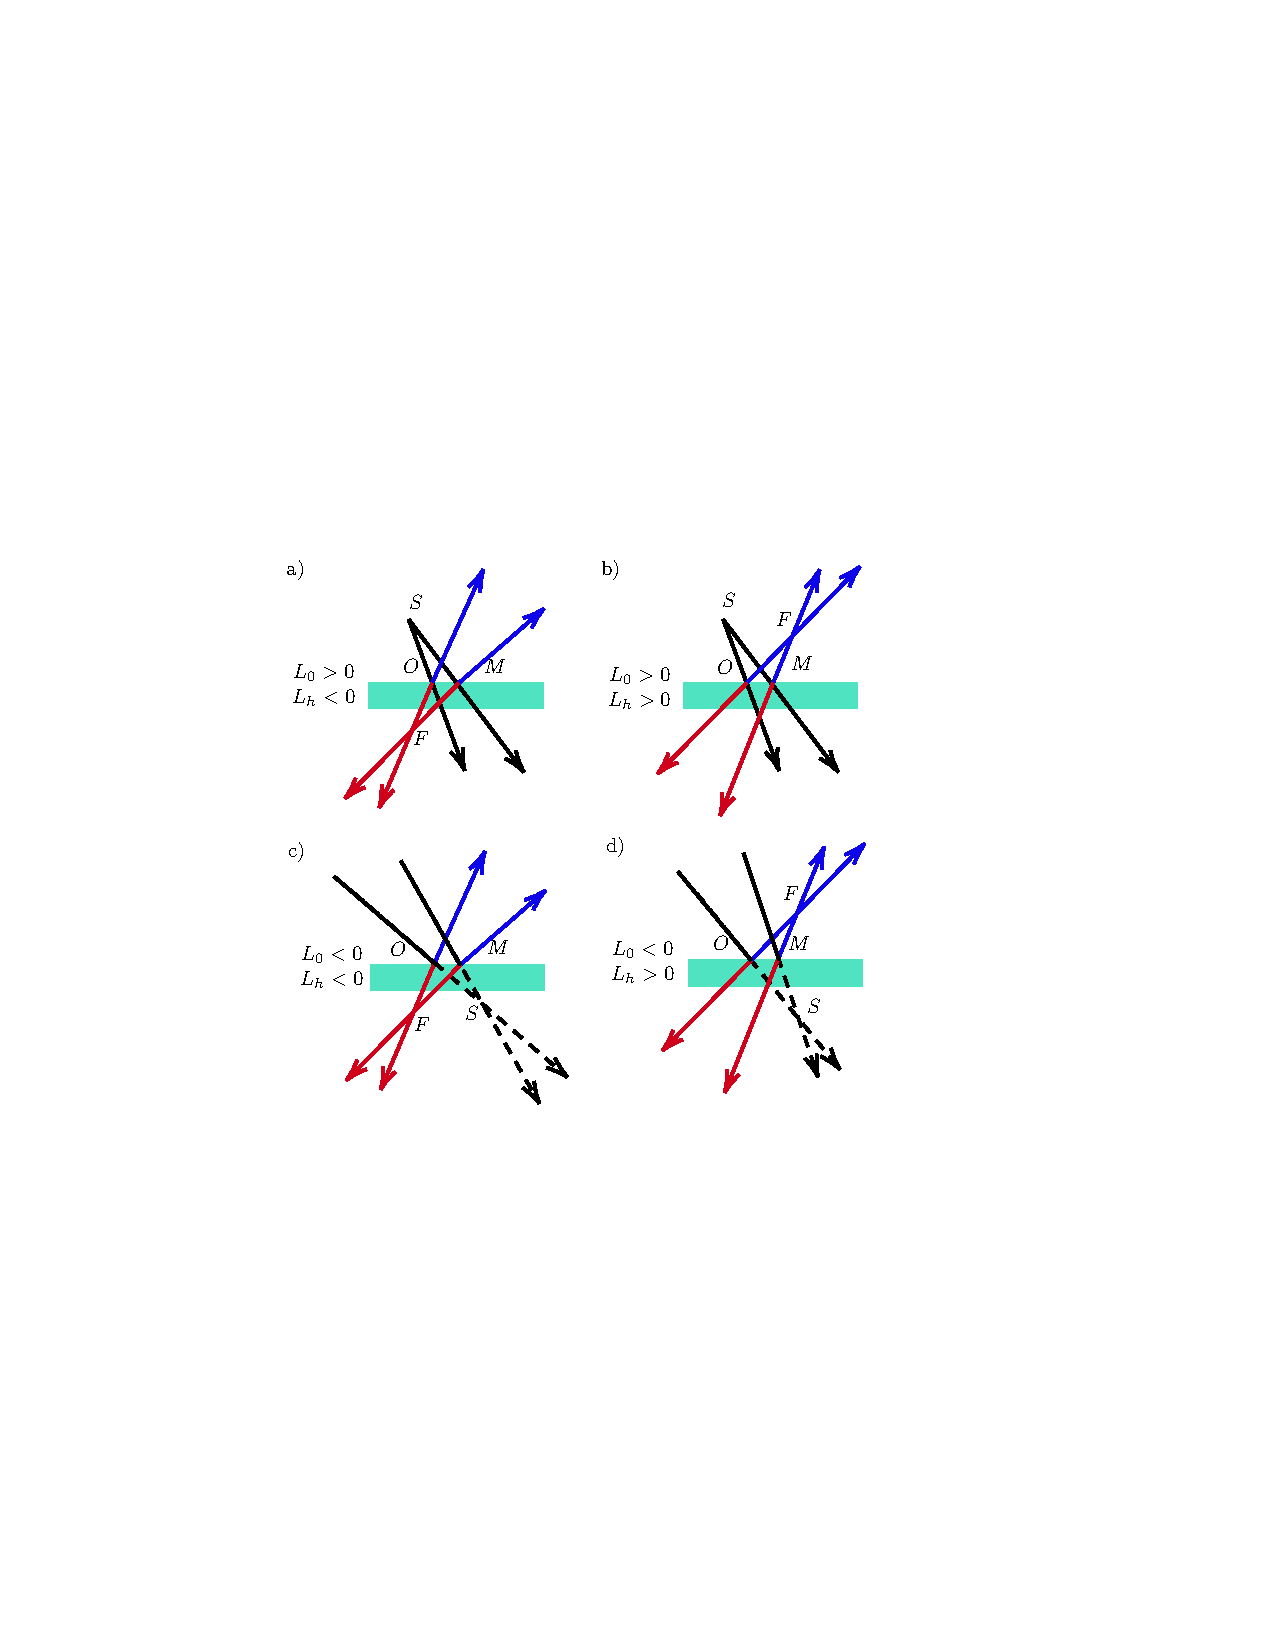
\includegraphics{fig1}
% \end{figure}


\end{document}                    % DO NOT DELETE THIS LINE
%%%%%%%%%%%%%%%%%%%%%%%%%%%%%%%%%%%%%%%%%%%%%%%%%%%%%%%%%%%%%%%%%%%%%%%%%%%%%%
